\documentclass[12pt]{article}
\usepackage{amsmath,amsthm,amssymb,amsfonts,fullpage,verbatim,bm,graphicx,enumerate,epstopdf,lscape,enumitem}
\usepackage[titletoc,title]{appendix}
\usepackage[dvipsnames,usenames]{color}
\usepackage[pdftex,pagebackref,colorlinks=true,pdfpagemode=UseNone,urlcolor=blue,linkcolor=blue,citecolor=BrickRed,pdfstartview=FitH,plainpages=true]{hyperref}
\usepackage[top=1.15in,bottom=1.15in,left=1.25in,right=1.25in,letterpaper]{geometry}
\usepackage[font=scriptsize]{caption}
\usepackage{caption,subcaption}

\setlist{noitemsep}

\def\CC{\mathbb{C}}
\def\RR{\mathbb{R}}
\def\ZZ{\mathbb{Z}}
\def\PP{\mathbb{P}}
\def\EE{\mathbb{E}}
\def\II{\mathbb{I}}


\newcommand{\Ga}{\alpha}
\newcommand{\Gb}{\beta}
\newcommand{\Gg}{\gamma}     \newcommand{\GG}{\Gamma}
\newcommand{\Gd}{\delta}     \newcommand{\GD}{\Delta}
\newcommand{\Ge}{\epsilon}
\newcommand{\Gf}{\phi}       \newcommand{\GF}{\Phi}
\newcommand{\Gh}{\theta}
\newcommand{\Gi}{\iota}
\newcommand{\Gk}{\kappa}
\newcommand{\Gl}{\lambda}    \newcommand{\GL}{\Lambda}
\newcommand{\Go}{\omega}     \newcommand{\GO}{\Omega}
\newcommand{\Gs}{\sigma}     \newcommand{\GS}{\Sigma}
\newcommand{\Gt}{\tau}
\newcommand{\Gz}{\zeta}
\newcommand{\s}{\sigma}
\newcommand{\tr}{\triangle}


\begin{document}

\title{\textbf{Title}}
\date{}
\maketitle

\section{Abstract}
\section{Introduction}
In recent years, various shrinkage and thresholding procedures have become ever more popular in many applications where sparsity is desired. Here ``sparsity'' is loosely defined in that it also includes the case where many terms are near-zero, as opposed to exactly zero. The most prominent usage of such procedures appear in multiresolution denoising analyses such as wavelets, where sparsity in a transformed domain often corresponds to smoothness in the data space [references]. Other examples include estimation of covariance and precision matrices (though thresholding is used more often here since zero terms are actually desired) [references], accounting for different measurement precisions in FDR control for multiple testing [references], or more generally optimizing penalized likelihood problems such as LASSO [references]. In this paper we will look at a flexible and adaptive shrinkage method named ASH, and illustrate its value in two key areas of univariate wavelet denoising.

Before delving deeper into the two denoising tasks, we first present a brief overview of wavelet estimators. These estimators have become extremely popular in nonparametric regression problems following the seminal paper by Donoho \& Johnstone (1994). Wavelet methods are locally adaptive in that they achieve the optimal minimax rate over a wide variety of functions, yet are also computationally faster than many other adaptive methods such as variable-bandwidth kernel methods [antoniadis 2001]. While classical thresholding estimators have been shown to possess optimal asymptotic properties, an extensive simulation study by Antoniadis et al. (2001) has demonstrated that various Bayesian shrinkage methods are usually more adaptive than thresholding methods in finite samples, outperforming the latter in terms of mean squared error (MSE). However, many Bayesian methods require specific distributional assumptions, and are not easily extensible to more complex problems, two of which we subsequently describe. On the other hand, our method simplies the task by making approximations, while still possessing good finite sample performance and computational efficiency. These approximations also allow us to use ASH as the common shrinkage procedure in both the problems.

The first problem relates to mean and variance estimation with Gaussian noise. Although the framework for homoskedastic Gaussian errors has been thoroughly developed in the wavelet literature [references], existing methods dealing with heteroskedastic errors have been far and few between. Fan \& Yao (1998) estimated the variance by smoothing the squared residuals using local polynomial smoothing, while Brown \& Levine (2007) employed difference-based kernel estimators. Making use of the local adaptivity of wavelet methods, Cai \& Wang (2008) improved upon previous variance estimation methods using a wavelet thresholding approach on first order differences. Here we present an approach that estimates both the mean and variance accurately by incorporating ASH into a novel wavelet denoising framework. [mention the lack of available software?]

The second task is to denoise a Poisson distributed signal. This often occurs in the experimental sciences such as gamma-ray burst signals in astronomy [references], and more recently in genetics where high throughput sequencing data is of interest. This problem is interesting because there are many distinct ways to perform signal recovery. Variance stabilizing techniques together with normal approximations have been proposed by Donoho (1993) and Fryzlewicz \& Nason (2001), by exploiting the mean-variance relationship of a Poisson distribution. Kolaczyk (1997, 1999a) derived thresholds achieving optimal asymptotic properties in the context of wavelet transformations, similar to the thresholds in the i.i.d. Gaussian case.  However, variance stabilizing methods are computationally inefficient due to the presence of external cycle-spinning, and threshold-based methods may not result in satisfactory finite sample performance. Furthermore, both these methods are quite sensitive to the choice of the primary resolution level as our simulations will show. Multiscale analysis using recursive dyadic partitions within a Bayesian framework was later developed by Kolaczyk (1999b) to make use of a particular form of likelihood factorization, but a relatively inflexible conjugate prior was chosen. We will improve upon the prior (and likelihood) specification by using ASH as the main shrinkage procedure in a Bayesian framework similar to that of Kolaczyk (1999b).

Both the aforementioned problems are harder to deal with than the classical problem with i.i.d. Gaussian errors, and usually requires extension of the ideas from the latter task. Before proceeding to describe the two problems in detail, we will first describe briefly the portion of ASH that performs shrinkage. 

As a generic shrinkage method, ASH takes as input a vector of estimates $\hat{\Gb}_i,i=1,...,n$ and their standard errors $\hat{\s}_i\equiv se(\hat{\Gb}_i),i=1,...n$, and outputs shrunken estimates of $\bm{\Gb}$. Specifically, the likelihoods for the true parameters $\Gb_i,i=1,...n$ are assumed to be i.i.d. $N(\Gb_i;\hat{\Gb}_i,\hat{\s}_i^2)$. ASH then assumes exchangeability of the $\Gb_i$'s and sets the following ``shrinkage'' prior on $\Gb_i$ for each $i$:
\begin{eqnarray}
\Gb_i|\bm{\pi}=\sum_{k=1}^m \pi_k N(\Gb_i;0,s_k^2)
\end{eqnarray}
Note that $\bm{\pi}$ and $\bm{s}^2$ are shared across all the $\Gb_i$'s, allowing one to borrow information across all observations. The full likelihood for $\bm{\pi}$ given $\bm{\hat{\Gb}}$ and $\bm{\hat{\s}}$ is then a product of likelihoods for $\bm{\pi}$ given each $\hat{\Gb}_i$ and $\hat{\s}_i$. Since the likelihoods are Gaussian and the priors are mixtures of Gaussians, the posterior distribution of $\Gb_i$ given $\hat{\Gb}_i$ and $\bm{\hat{\pi}}$ is analytically tractable, where the mixing proportions $\bm{\hat{\pi}}$ are maximum likelihood estimates. The posterior mean of $\Gb_i$ is taken to be the point estimate of $\Gb_i$, resulting in shrinkage.

The flexibility and computational efficiency of ASH is immediately obvious, which motivates us to extend this method to the more complex wavelet settings described here. As an Empirical Bayes procedure, ASH borrows information across all available data and is extremely data adaptive. At the same time, the key advantage of ASH over other Empirical Bayes procedures such as EbayesThresh [Johnstone \& Silverman (2005)] and the commonly used ``spike-and-slab'' prior (is there a reference for this?) is that variable variances are allowed as input, a feature which latter methods lack. This is also the primary reason we can use ASH as the only shrinkage procedure in both the problems described above. Furthermore, Gaussian mixtures can effectively approximate any unimodal distribution, allowing for an extremely flexible prior. In tackling these two specific problems, we can speed up the entire signal denoising problem via likelihood approximations (discussed in the next section), allowing our method to be computationally efficient without compromising accuracy. Typical wavelet methods require the specification of a primary resolution level as a ``tuning'' parameter, which could substantially influence the accuracy of the method. However, applying ASH to every resolution in the wavelet transformationwe spares us the need for such a parameter. For an in-depth understanding of the original motivations and applications of ASH, see Stephens (??). With the main shrinkage method accounted for, we will proceed to explore the two aforementioned problems in detail. Note that one only needs to supply a vector of estimates $\hat{\Gb}$ and their standard errors se$(\hat{\Gb})$ to ASH to obtain posterior estimates; hence, we will focus on obtaining these estimates and standard errors when describing our methods.
\section{Method}
\subsection{Gaussian denoising with heteroskedastic errors}
Consider the nonparametric regression model with i.i.d. Gaussian errors:
\begin{eqnarray}\label{eq:1d gaussian model}
Y_i=\mu_i+\Ge_i
\end{eqnarray}
for $i=1,...,n$, where $\bm{Y}$ is the vector of observations, $\bm{\mu}$ is the mean curve, and $\Ge_i$ are independent $N(0,\s^2)$ noise. Assume that $n=2^J$ for some integer $J$, as is standard in the wavelet literature. To motivate our method, we first describe wavelet shrinkage from a Bayesian perspective.

The wavelet coefficients $\bm{d}$ are given by
\begin{eqnarray}
\bm{d}=W\bm{Y}
\end{eqnarray}
where $W$ denotes the orthogonal $n\times n$ matrix corresponding to the orthonormal wavelet basis chosen.
Since $\mathbb{V}(Y)=\s^2I$,
\begin{eqnarray}\label{eq:waveletcoef}
\bm{d}\sim N_n(\bm{\Ga},\s^2I)
\end{eqnarray}
where $\bm{\Ga}=W\mathbb{E}(\bm{Y})$. This implies that the likelihood for $\bm{\Ga}$ factorizes into a product of likelihoods for $\Ga_i$, $i=1,...,n$. As such, a natural and computationally convenient approach is to set independent priors on $\Ga_i$ as a form of ``shrinkage''. Here we apply the priors from ASH to each resolution level separately, resulting in
%Although there are many choices for the prior, we use the Gaussian mixture prior from ASH in our method, given by
\begin{eqnarray}\label{eq:ashprior}
\Ga_{jk}=\sum_{l=1}^m \pi_l^{(j)} N(0,(s_l^{(j)})^2)
\end{eqnarray}
with $\sum_l \pi_l^{(j)}=1$, for $j=1,...,J$. $\pi_i^{(j)}$ and $(s_i^{(j)})^2$ are hyperparameters that are shared between coefficients in the same resolution level, and $m$ is the number of mixture components. In ASH, $m$ is usually chosen to reasonably approximate any unimodal distribution, while maintaining an acceptable computational speed. Note that, for notational convenience, we have switched to a double index following standard wavelet convention for indices: here $j=1,...,J$ is the resolution level, and $k=0,...,2^j-1$ is the location within each resolution level $j$. By applying the inverse wavelet transform to the posterior mean $\hat{\bm{\Ga}}$ that ASH produces, one can obtain the posterior mean of $\bm{\mu}$, which serves as an estimate that minimizes the MSE. One could also construct credible bands using the posterior variances.

While many existing methods perform well in the presence of i.i.d. (Gaussian) errors, heteroskedastic (but still independent) errors present a different challenge. One key obstacle when dealing with heteroskedastic errors is that the likelihood for $\bm{\Ga}$ does not necessarily factorize. Given the true variances and hence the likelihood, one could compute the full posterior distribution using some specified prior. However, this would be computationally cumbersome, and may be infeasible when extended to multiple signals or higher dimensions. In this case, a suitable prior might also be difficult to find. As such, one key aspect of our approach is to treat the wavelet coefficients as if they were independent, so that the true likelihood is approximated by a composite likelihood (see Silverman (1999) for an example where this is done).

To describe our approach in more detail, first assume that the true variance function is known and given by $\mathbb{V}(\Ge_i)=\s_i$, and that the true mean function is given by $\bm{\mu}=(\mu_1,...,\mu_t)$, where $T=2^J$ for some positive integer $J$. Hence
\begin{eqnarray}
\bm{Y}\sim N_n(\bm{\mu},\Sigma)
\end{eqnarray}
where $\Sigma=\textrm{diag}(\s_1,...,\s_T)$ is a diagonal matrix. For the rest of this subsection, we will use the non-decimated wavelet transform (NDWT) instead of the standard DWT to achieve translation invariance. This in turn reduces the presence of artifacts, which often occur near discontinuities in the underlying signal (see eg. Coifman \& Donoho (1995)). Then,
\begin{eqnarray}
\bm{d}\sim N_n(\bm{\Ga},\tilde{\Sigma})
\end{eqnarray}
where $\bm{d}$ is the vector of detail coefficients, $\bm{\Ga}=W\bm{\mu}$, and $\tilde{\Sigma}=W\Sigma W^T$, where $W$ is the matrix associated with the NDWT for a given wavelet basis. By treating the likelihood for $\bm{\Ga}$ as if it were independent, it can be written as follows(using the double index mentioned above):
\begin{eqnarray}\label{eq:likelihood}
L(\bm{\Ga}|\bm{d})=\prod_{j=0}^J\prod_{k=0}^{T-1}P(d_{jk}|\Ga_{jk})
\end{eqnarray}
where $P(d_{jk}|\Ga_{jk})=\phi(d_{jk};\Ga_{jk},\tilde{\Sigma}_{(jk,jk)})$. Note that there are $n$ coefficients at each resolution level instead of $2^j$ for resolution $j$ due to the NDWT. Here $\phi$ denotes the Gaussian density function. Since $\Sigma$ is diagonal, it is easy to see that $\tilde{\Sigma}_{(jk,jk)}=\sum_{i=1}^T \Sigma_{ii}W_{jk,i}^2$. In our method, we use ASH to assign independent priors to $\Ga_{jk}$ as with \eqref{eq:ashprior}. %ASH also allows us to estimate the $\pi_i$'s via a maximum likelihood approach and fix the $\s_i$'s by using a grid of values. This particular choice of prior specification is extremely flexible, being able to approximate any symmetrical zero-centered distribution, as well as allowing for a relatively easy estimation of the hyperparameters through empirical Bayes. See ASH for more details regarding this choice of prior (?)
While ASH produces shrunken estimates of $\Ga_{jk}$ for $j,k>0$, we estimate $\Ga_{00}$ using the corresponding scaling coefficient, which seems intuitively appealing. Finally, we can obtain an estimate of $\mu$ by using the average basis inverse, which is essentially an average of the inverse wavelet transforms for every shift of the data (see Coifman \& Donoho (1995)) since we are using the NDWT. Although the method described here uses a matrix formulation for easier conceptual understanding, the actual NDWT and inverse transform are done through Mallat's pyramid algorithm, taking only $n\log(n)$ time.

Though we have assumed that the true variances were known for mean estimation, the problem of variance estimation itself is a non-trivial one. Here we make the reasonable assumption that the variance function is also spatially structured, in addition to the mean function. The approach we took is similar in spirit to that of Cai \& Wang (2008), making use of wavelet decomposition as well. However, while they use first order differences, we look at the squared residuals. As such, we need a reasonably accurate estimator of the mean function to form sensible residuals. For clarity of presentation, we will first assume that the true mean function is known. Define
\begin{eqnarray}\label{eq:varobs1}
Z_i^2=(Y_i-\mu_i)^2
\end{eqnarray}
to be the ``observations'' for the unknown variance function. Note that $\mathbb{E}(Z_i^2)=\s_i^2$, so that $Z_i^2$ is unbiased for the true variance at point $i$. At this point we can treat this as yet another mean estimation problem, with the added complication that the variance of $Z_i^2$ has a $\chi^2$ distribution squared. To simplify the problem, we approximate this likelihood by a Gaussian likelihood. Of course, better likelihoods and priors could be used that reflect the skewness in the distributions of the ``observations'', but we found that a normal approximation works reasonably well (especially for smoother variance functions), and has the key advantage of being easy and fast to implement. The variance estimation process is then very similar to one for mean estimation as described above, with a few extra details. The full procedure is outlined in Appendix \ref{app:var estimation}.

Now that we can estimate $\bm{\mu}$ given $\bm{\s}^2$ and vice versa, a natural procedure for jointly estimating $\bm{\mu}$ and $\bm{\s}^2$ is an iterative one. That is, we estimate $\bm{\mu}$ given some initial estimate of $\bm{\s}^2$, then estimate $\bm{\s}^2$ given the previous estimate of $\bm{\mu}$, and iterate the process. In our simulations, we have found that two cycles are usually sufficient to produce relatively accurate estimates. To start off the algorithmm, an initial estimate would be the square of first order differences between adjacent points, as discussed in previous variance estimation papers (eg Cai \& Wang (2008)). This estimator has the property that it is approximately unbiased for the variance at the two corresponding points, provided that the mean and the variance function is smooth enough. To be more specific, the initial variance estimates are defined by
\begin{eqnarray}\label{eq:initial var est}
\hat{\s}_i^2=\frac{1}{2}\left(\sum_{i=1}^n(Y_i-Y_{i-1})^2+\sum_{i=1}^n(Y_i-Y_{i+1})^2\right)
\end{eqnarray}
where $Y_0\equiv Y_n$ and $Y_{n+1}\equiv Y_1$, due to periodicity assumptions in wavelet methods. In summary, our approach for joint mean and variance estimation can be described in three steps:
\begin{enumerate}
\item Using squared first order differences \eqref{eq:initial var est} as estimates of $\bm{\s}^2$, estimate $\bm{\mu}$ as if $\bm{\s}^2$ was known (see above for the case when $\bm{\s}^2$ is known)
\item Given the estimate of $\bm{\mu}$, take squared residuals and treat those as ``observations'' for $\bm{\s}^2$. Next, project them into wavelet space and apply shrinkage to the wavelet coefficients, before projecting them back into data space to obtain an estimate of $\bm{\s}^2$.
\item Repeat steps (1)-(2) once to obtain the final estimates of $\bm{\mu}$ and $\bm{\s}^2$ respectively.
\end{enumerate}
\subsection{Poisson denoising}
Next we turn to another popular nonparametric regression problem and demonstrate how we could make use of ASH. Specifically, we again assume an underlying signal $\Gl_i$, $i=1,...,n$ with $n=2^J$ for some positive integer $J$. Further assume that each data point $Y_i$, $i=1,...,n$ is realized from a Poisson distribution with mean $\Gl_i$ ie. $Y_i=\textrm{Pois}(\Gl_i)$. Our goal is to recover the true intensity $\bm{\Gl}$ as accurately as possible, given $Y_k$. To make our approach easier to understand and relate it to wavelet-based methods, we first summarize the data in a recursive manner (see Kolaczyk (1999) and Nowak (1998):
\begin{eqnarray}Y_{Jk}\equiv Y_k\end{eqnarray}
for $k=1,...,n$, and
\begin{eqnarray}Y_{jk}=Y_{j+1,2k}+Y_{j+1,2k+1}\end{eqnarray}
for resolution $j=0,...,J-1$ and location $k=0,...,2^j-1$. Hence, we are summing more blocks of observations as we move to coarser levels. Another way to define the $Y$'s is
\begin{eqnarray}Y_{jk}=\sum_{l=k2^{J-j}+1}^{(k+1)2^{J-j}}Y_l\end{eqnarray}
for $j=0,...,J$ and $k=0,...,2^j-1$.
Further define the following:
\begin{eqnarray}\Gl_{Jk}\equiv \Gl_k\end{eqnarray}
for $k=1,...,n$, and
\begin{eqnarray}\Gl_{jk}=\Gl_{j+1,2k}+\Gl_{j+1,2k+1}\end{eqnarray}
for $j=0,...,J-1$ and $k=0,...,2^j-1$. Furthermore, define
\begin{eqnarray}\label{eq:poisson wc}\Ga_{jk}=\log(\Gl_{j+1,2k})-\log(\Gl_{j+1,2k+1})\\\end{eqnarray}
for $s=0,...,J-1$ and $l=0,...,2^j-1$. The ${\Ga}$'s defined this way is extremely similar to the (true) Haar wavelet coefficients, which forms the basis of our approach. Using this recursive representation, we can see that the likelihood for $\bm{\Ga}$ factorizes into a product of likelihoods, where $\bm{\Ga}$ is the vector of all the $\Ga_{sl}$'s. To be specific, we have
\begin{eqnarray}
L(\bm{\Ga}|\mathbf{Y})&=&P(\mathbf{Y}|\bm{\Ga})\\
&=&P(Y_{0,0}|\Gl_{0,0})\prod_{j=0}^{J-1}\prod_{k=0}^{2^j-1}P(Y_{j+1,2k}|Y_{j,k},\Ga_{j,k})\\
&=&L(\Gl_{0,0}|Y_{0,0})\prod_{j=0}^{J-1}\prod_{k=0}^{2^j-1}L(\Ga_{j,k}|Y_{j+1,2k},Y_{j,k})
\end{eqnarray}
where the factorization is due to the recursive definition above. Note that $Y_{00}|\Gl_{00}\sim \textrm{Pois}(\Gl_{00})$. For any given $j,k$, $Y_{jk}$ is a sum of two independent Poisson random variables, and is itself a Poisson random variable. Hence
\[Y_{j+1,2k}|Y_{jk},\Ga_{jk}\sim \textrm{Bin}({Y_{jk},\frac{1}{1+e^{-\Ga_{jk}}}\equiv\frac{\Gl_{j+1,2k}}{\Gl_{jk}}})\]
Kolaczyk (1999) set a conjugate shrinkage prior (a mixture of a point mass at 0.5 and a uniform distribution, similar to the ``spike and slab'' prior for the Gaussian case) for the parameters $\frac{\Gl_{j+1,2k}}{\Gl_{jk}}$ and used a Binomial likelihood. However, we work with the parameters $\Ga_{sl}$ as defined in \eqref{eq:poisson wc} and approximate the logit-Binomial (is there such a thing?) likelihoods by Gaussian likelihoods, and replace the two-component prior in Kolaczyk (1999) by the more flexible prior from ASH. Furthermore, these parameters can be more easily connected to the true wavelet coefficients since they consist of (log) differences rather than ratios.

To describe the approximation process in more detail, we drop the subscripts for notational convenience. One direct approximation of the likelihood for $\Ga$ is the Laplace approximation, which results in the Gaussian likelihood given by $\phi(\Ga;\hat{\Ga}_{MLE},\mathbb{V}(\hat{\Ga}_{MLE}))$. Here $\phi$ is the normal density function, and $\hat{\Ga}_{MLE}$ is the maximum likelihood estimator. We would then estimate $\mathbb{V}(\hat{\Ga}_{MLE})$ by the square of the asymptotic standard deviation for $\hat{\Ga}_{MLE}$. Specifically,
% for some appropriate estimator $\hat{\Ga}$. This choice of parameters for the Gaussian approximation is also appropriate in the sense that it minimizes the Kullback-Leibler divergence between a Gaussian distribution and the likelihood for $\Ga$ (also known as moment matching).

%We next consider appropriate estimators for the parameters $\Ga$ and $\sqrt{\mathbb{V}(\hat{\Ga})}$. The obvious choice would be the MLE of $\Ga$ and its asymptotic standard error respectively, given by
\begin{eqnarray}
\hat{\Ga}_{MLE}=\log(S/F)&\ \ \ S=0,...,N\\
se(\hat{\Ga}_{MLE})=\sqrt{SF/N}&\ \ \ S=0,...,N
\end{eqnarray}
where $S$ is the number of successes in the binomial setup, and $F=N-S$ is the number of failures (in our case the even locations would be successes and odd locations failures). The MLE has one notable drawback however, in that it cannot deal well with extreme cases. This would in turn affect the likelihood approximation in a non-negligible way. To improve the accuracy of the approximation at the endpoints of the binomial distribution (ie. when we have $\hat{p}=0$ or $N$, so that $\hat{\Ga}=-\infty$ or $\infty$ respectively), we instead aim to find a suitable estimator $\hat{\Ga}$ for $\Ga$. Next, we approximate the distribution of $\hat{\Ga}$ by a Gaussian distribution, so that the likelihood for $\Ga$ is automatically Gaussian, given by $\phi(\Ga;\hat{\Ga},\mathbb{V}(\hat{\Ga}))$. To that end, our final estimator will still be the MLE, but with Tukey's modification (Gart \& Zweifel (1967)) at the endpoints where $S=\{0,N\}$. Specifically, the estimator for $\Ga$ and its standard error are given by
\begin{eqnarray}\label{eq:pseudoMLE1}
&&\hat{\Ga}=\left\{
\begin{array}{lll}
\log\{(S+0.5)/(F+0.5)\}-0.5&\ \ \ S=0\\
\log\{S/F\}&\ \ \ S=1,2,...,N-1\\
\log\{(S+0.5)/(F+0.5)\}+0.5&\ \ \ S=N\\
\end{array}
\right.\\ \label{eq:pseudoMLE1se}
&&se(\hat{\Ga})=\sqrt{V^*(\hat{\Ga})-\frac{1}{2}\{V_3(\hat{\Ga})\}^2\left\{V_3(\hat{\Ga})-\frac{4}{N}\right\}}
\end{eqnarray}
where
\begin{eqnarray}
&&V_3(\hat{\Ga})=\frac{N+1}{N}\left(\frac{1}{S+1}+\frac{1}{F+1}\right)\ \ \ S=0,...,N\\
\label{eq:pseudoMLE2}&&V^*(\hat{\Ga})=V_3(\hat{\Ga})\left\{1-\frac{2}{N}+\frac{V_3(\hat{\Ga})}{2}\right\}
\end{eqnarray}
The square of the standard error in \eqref{eq:pseudoMLE1se} corresponds to $V^{\ast\ast}$ from p. 182 of Gart \& Zweifel (1967), and is chosen because it is less biased for the true variance of $\hat{\Ga}$ (when $N$ is small) as compared to the asymptotic variance of the MLE (see Gart \& Zweifel (1967)). The other two variance estimators from Gart \& Zweifel (1967), $V_1^{++}$ and $V^{++}$, were also considered in simulations and gave similar results, but $V^{\ast\ast}$ was chosen for its simple form.

Finally, the Delta method is used to reconstruct the signal in the original space from the posterior distribution of the $\Ga$'s (which are in the logit space). For full details on the reconstruction process as well as the Delta method, see Appendix \ref{app:reconstruction}.
\section{Simulations}
We now seek to validate the advantages of our method, named ``SMASH'', via simulation studies. To thoroughly investigate the performance of SMASH, we consider the Gaussian and Poisson cases separately. 

For the Gaussian case, we focus our attention mostly on mean estimation. Different test functions, sample sizes, signal-to-noise ratios (SNR) and variance functions were considered, to ensure that SMASH behaves well in a variety of settings. However, only a small portion of the results will be shown here to highlight key findings from the rather extensive simulation study. Full results from the study can be found \textcolor{red}{state where?}.  

To demonstrate the robustness of SMASH, we first consider homoskedastic errors. Due to the large number of methods available in the literature for this setting, we chose only a subset. The methods we considered in our simulation are discussed in detail in Antoniadis et al. (2001), and in particular Translation Invariant (TI) thresholding by Coifman \& Donoho (1995) performed the best on average, where performance is measured by mean squared error (MSE). We also considered the popular Empirical Bayes shrinkage procedure by Johnstone \& Silverman (2005), called Ebayesthresh. Figure \ref{fig:gaus_homo_comp} shows the mean integrated squared errors (MISEs) of SMASH, TI-thresholding, and Ebayesthresh for the ``Spikes'' mean function, with a signal to noise ratio of 3 and sample size 1024; figure \ref{fig:gaus_homo_comp} compares the MISEs of SMASH with two different options for the same scenario: the first assumes the default and hence estimates the mean without any assumptions on the variance function, while the second estimates the mean given the true variance function. The figures clearly indicate that the performance of SMASH is not impacted by the lack of explicit assumptions imposed on the variance function: it outperforms two of the most accurate wavelet denoising algorithms for i.i.d. Gaussian noise even when the i.i.d. assumption holds, and performs nearly as well as when the variance function is known, which is the best-case scenario for any denoising technique. These results also extend to other mean functions, SNRs and sample sizes.

\begin{figure}[ht]
\centering
	   \begin{subfigure}[b]{0.45\textwidth}
        \centering
        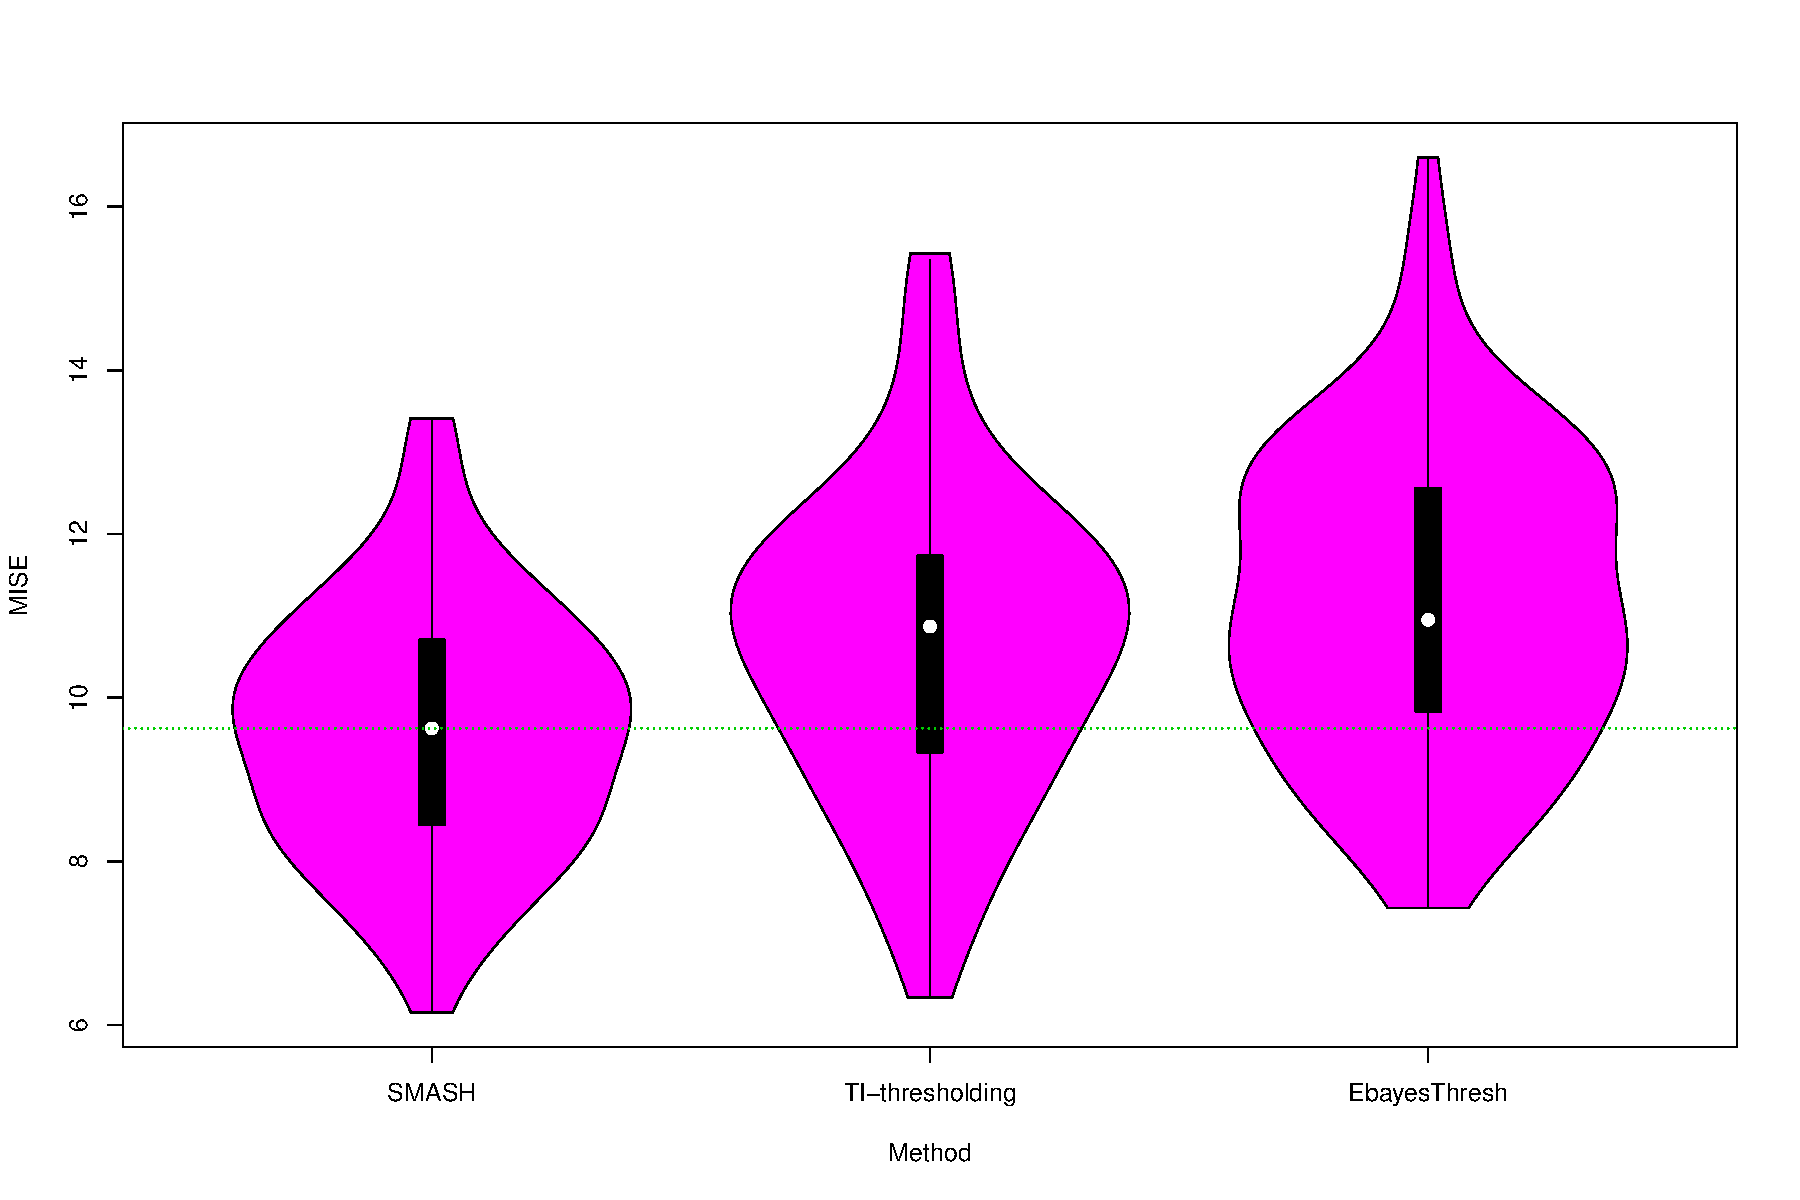
\includegraphics[width=\textwidth]{violin_gaus_homo_comp.pdf}
        \caption{}
        \label{fig:gaus_homo_comp}
    \end{subfigure}
    \hfill
    \begin{subfigure}[b]{0.45\textwidth}
        \centering
        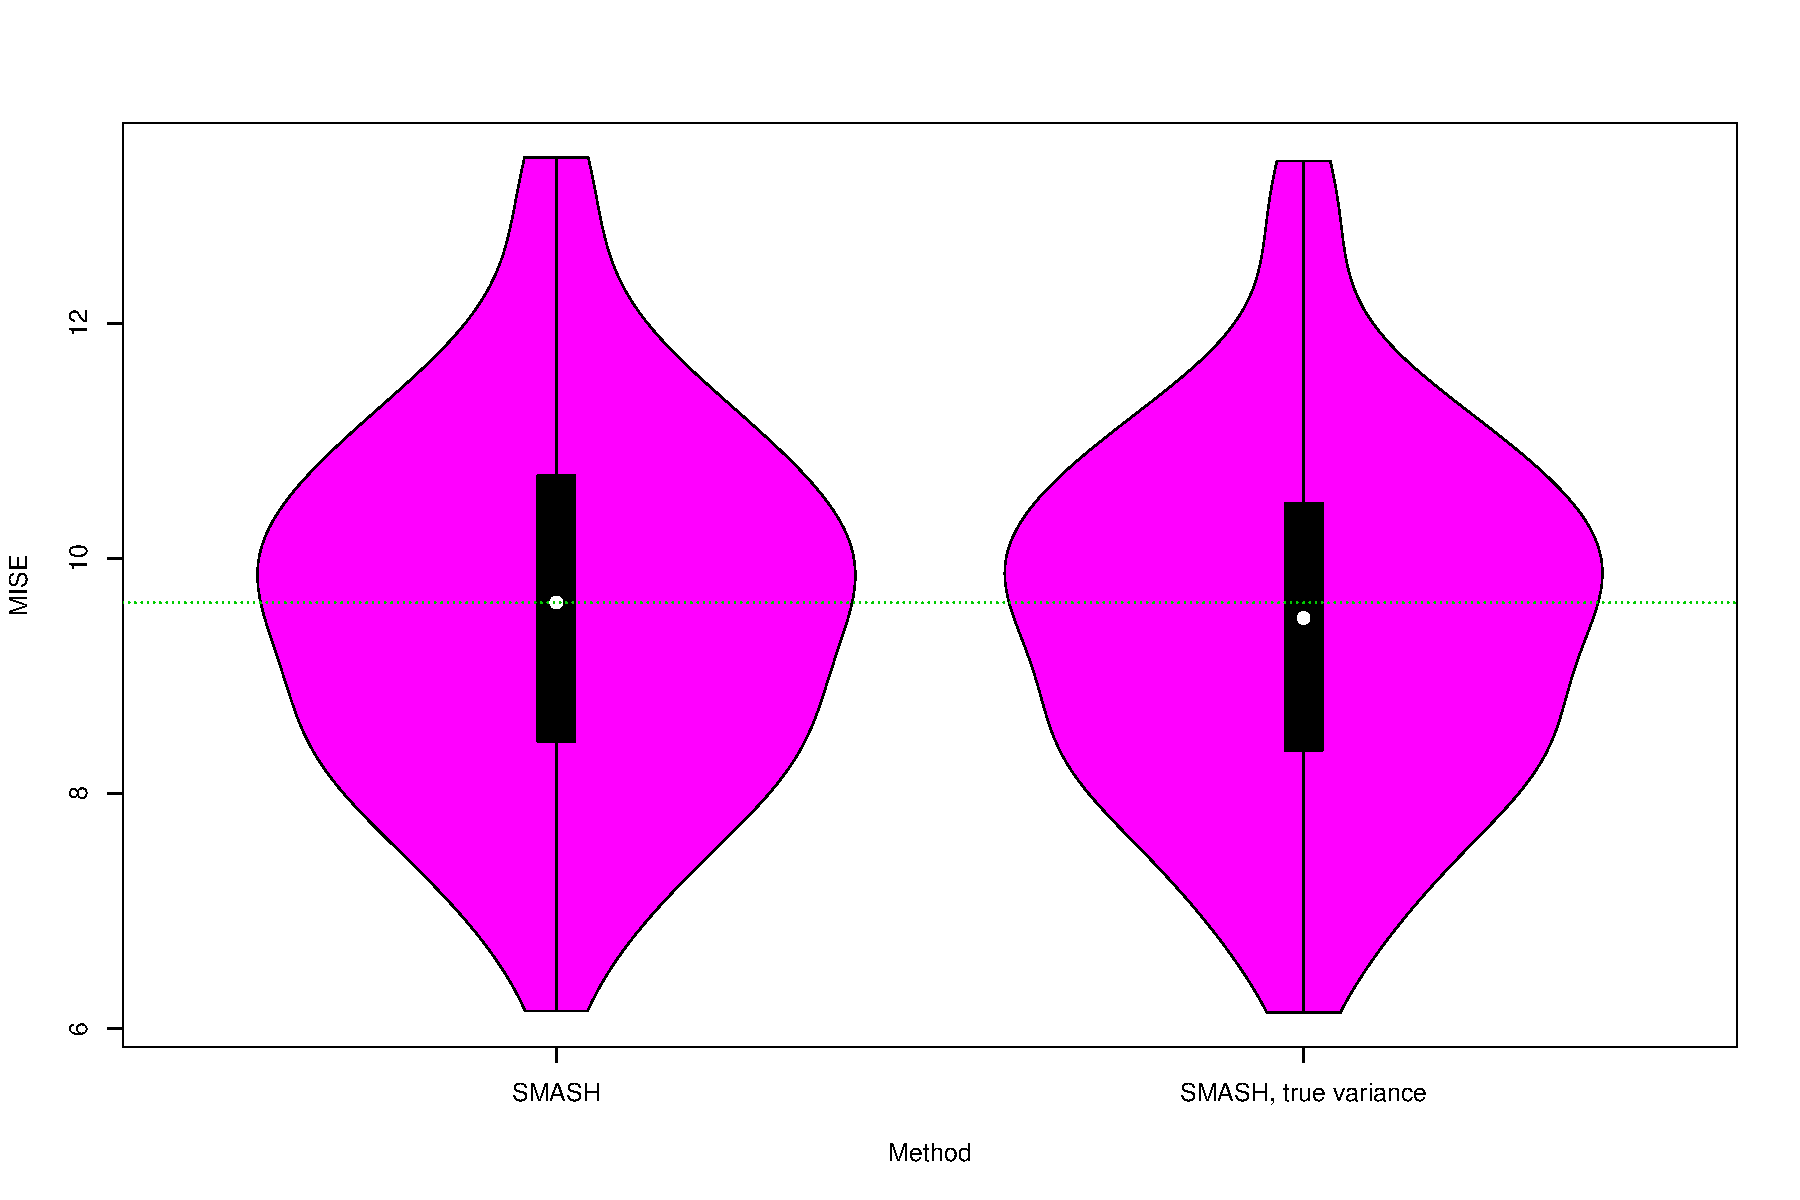
\includegraphics[width=\textwidth]{violin_gaus_homo_smash.pdf}
        \caption{}
        \label{fig:gaus_homo_smash}
    \end{subfigure}
    \caption{Violin plots of MISEs for various methods. Dashed green line indicates the median MISE for SMASH. a) compares SMASH against two popular and accurate denoising methods: TI-thresholding and Ebayesthresh, and b) demonstrates the performance gain of SMASH when it is provided the true variance.}
    \label{fig:gaus_homo}
\end{figure}

Having shown that SMASH performs well in the homoskedastic case without any explicit assumptions on the Gaussian noise, we now demonstrate its performance gain when the errors are heteroskedastic. Figure \ref{fig:simple_eg} demonstrates that SMASH is able to better capture the true signal than TI-thresh (with variance estimated by running median absolute deviation (RMAD)) on a simple simulation. For the sake of presentation, figure \ref{fig:gaus_hetero} highlights only the results from SMASH, TI-thresh (with various choices of variance estimation) and EbayesThresh for the ``Spikes'' mean function, with the ``Clipped Blocks'' variance function, a SNR of 3 and a sample size of 1024. Nevertheless, similar results hold in general for different mean and variance functions, SNRs, and sample sizes. 
\begin{figure}[ht]
\centering
	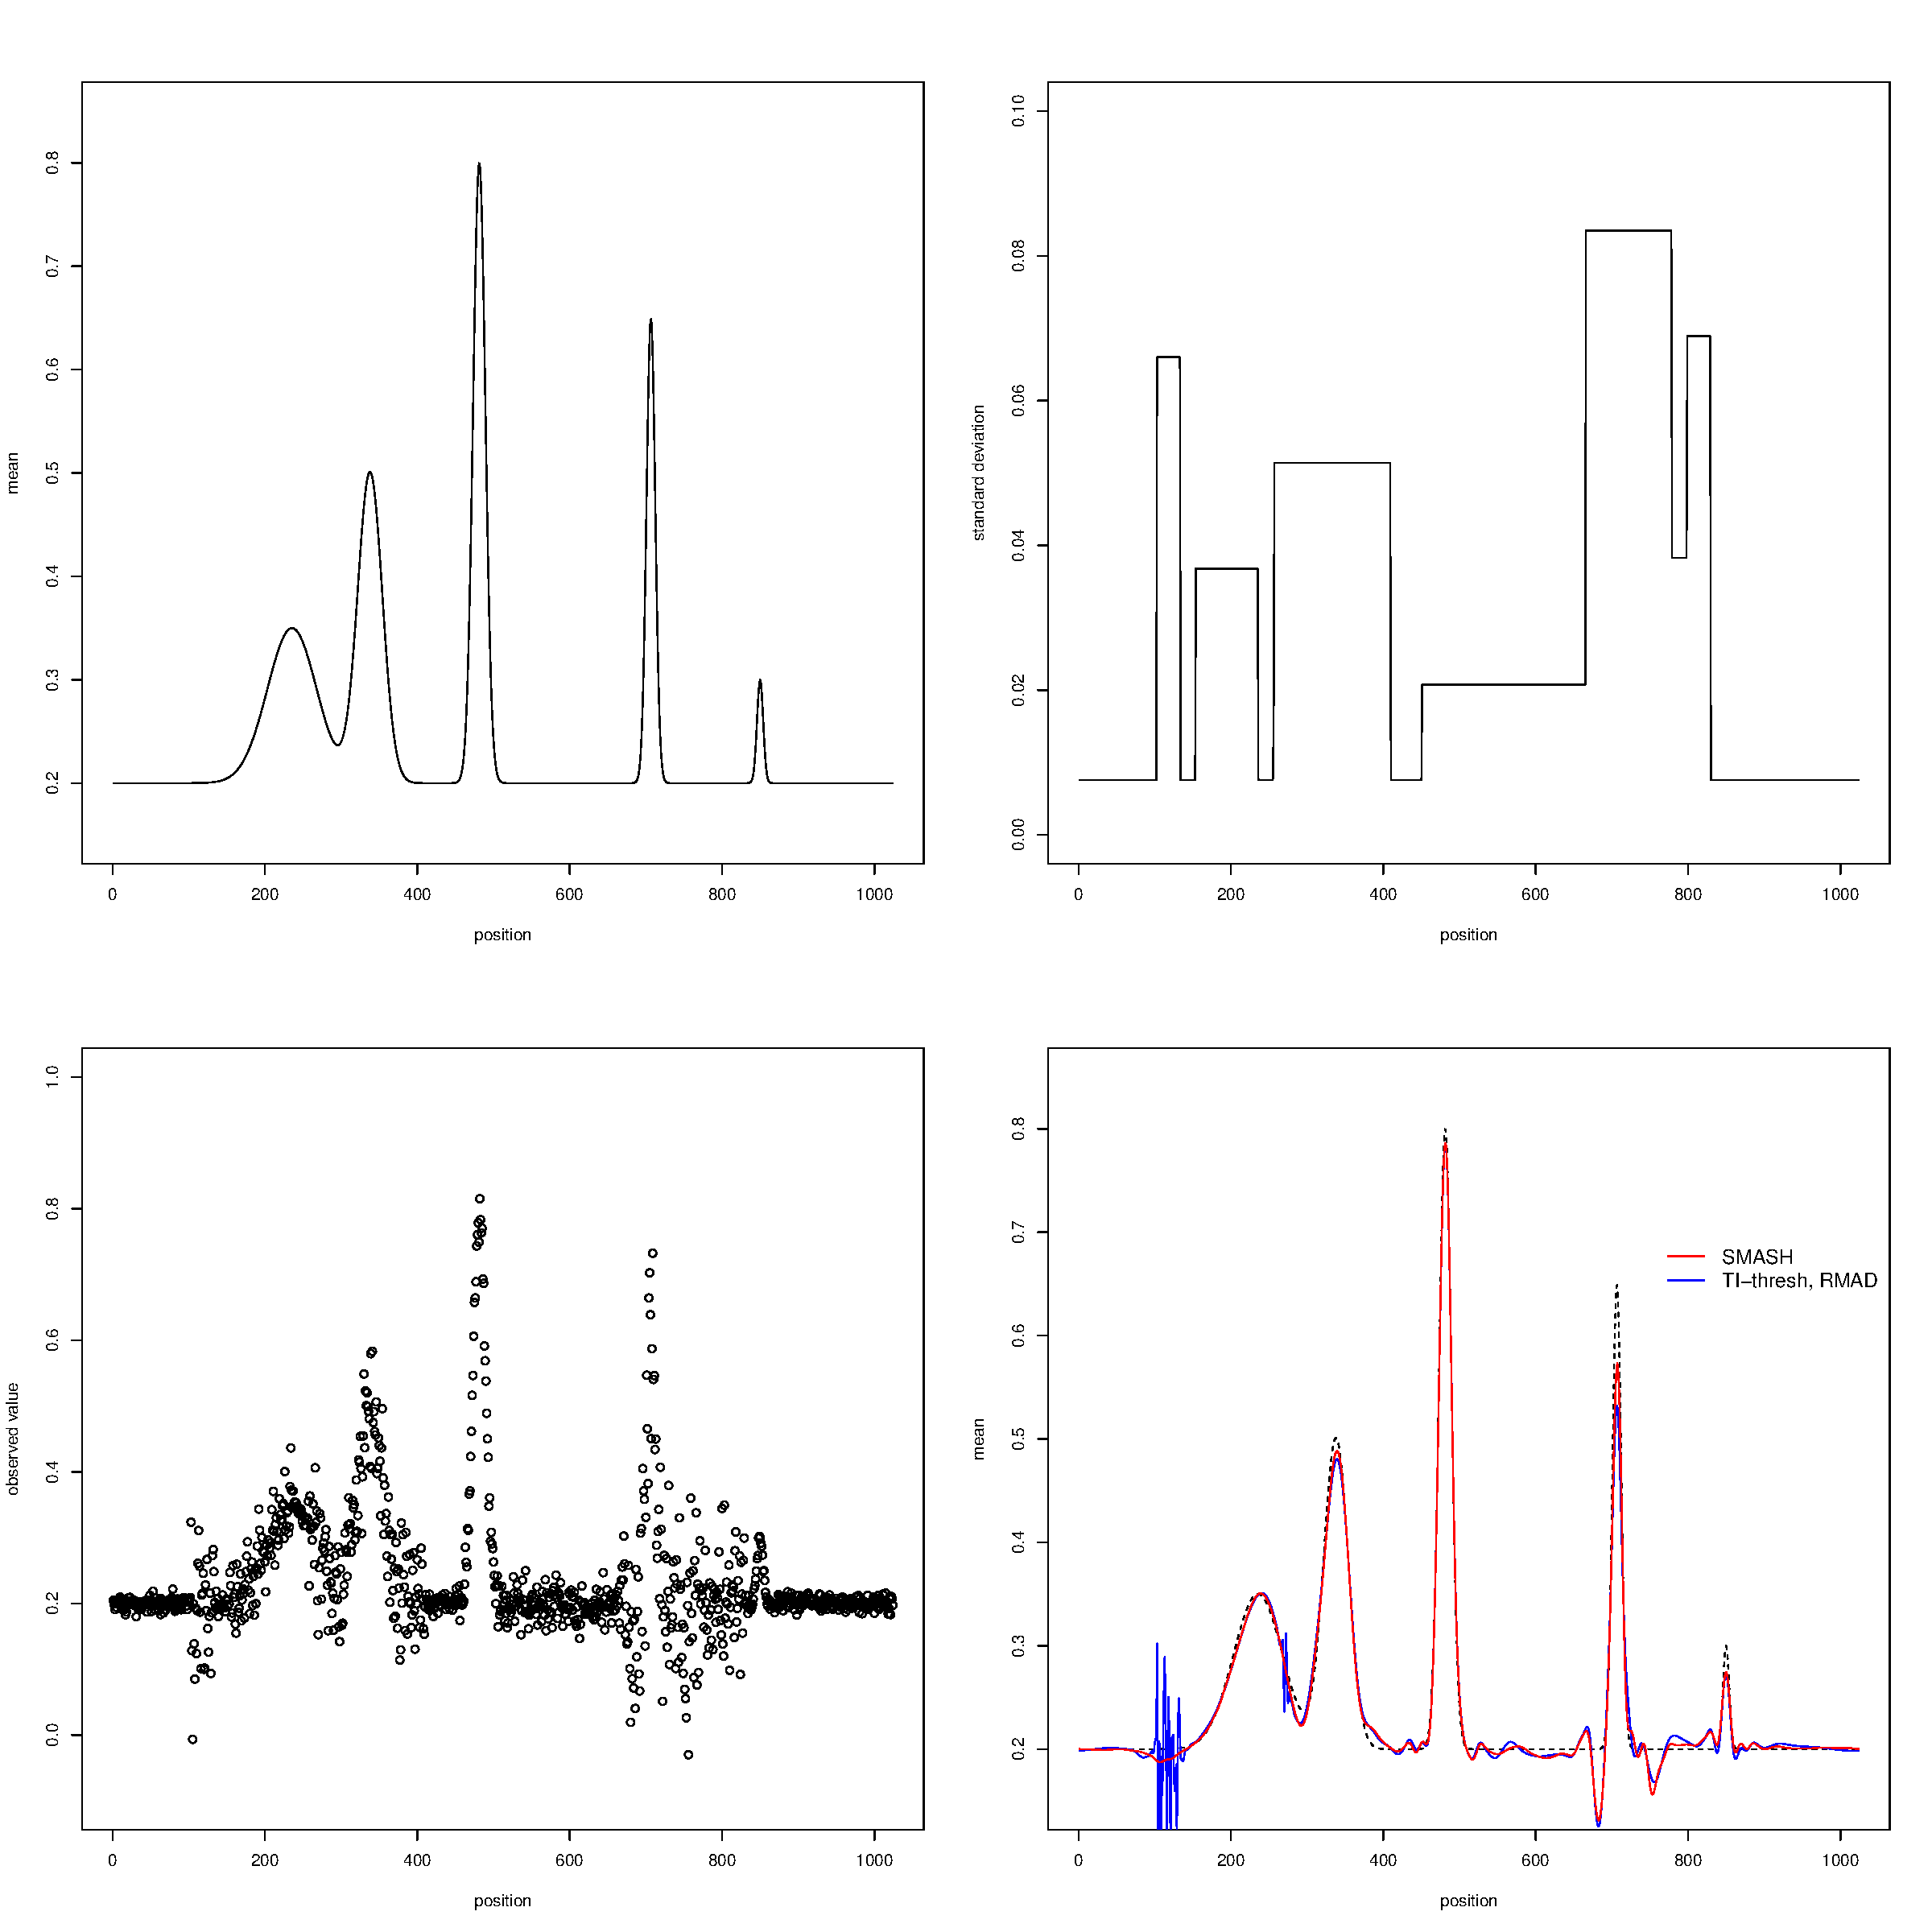
\includegraphics[width=\textwidth]{simple_eg.pdf}
	\caption{Simple illustration of heteroskedastic Gaussian denoising. Top left plot shows the mean function, top right plot shows the variance function, bottom left plot shows a sample dataset, and bottom right plot shows the estimated mean functions from SMASH and TI-thresh against the true mean function.}
	\label{fig:simple_eg}
\end{figure}    

%\begin{figure}[ht]
%\centering
    %\begin{subfigure}[b]{0.45\textwidth}
        %\centering
        %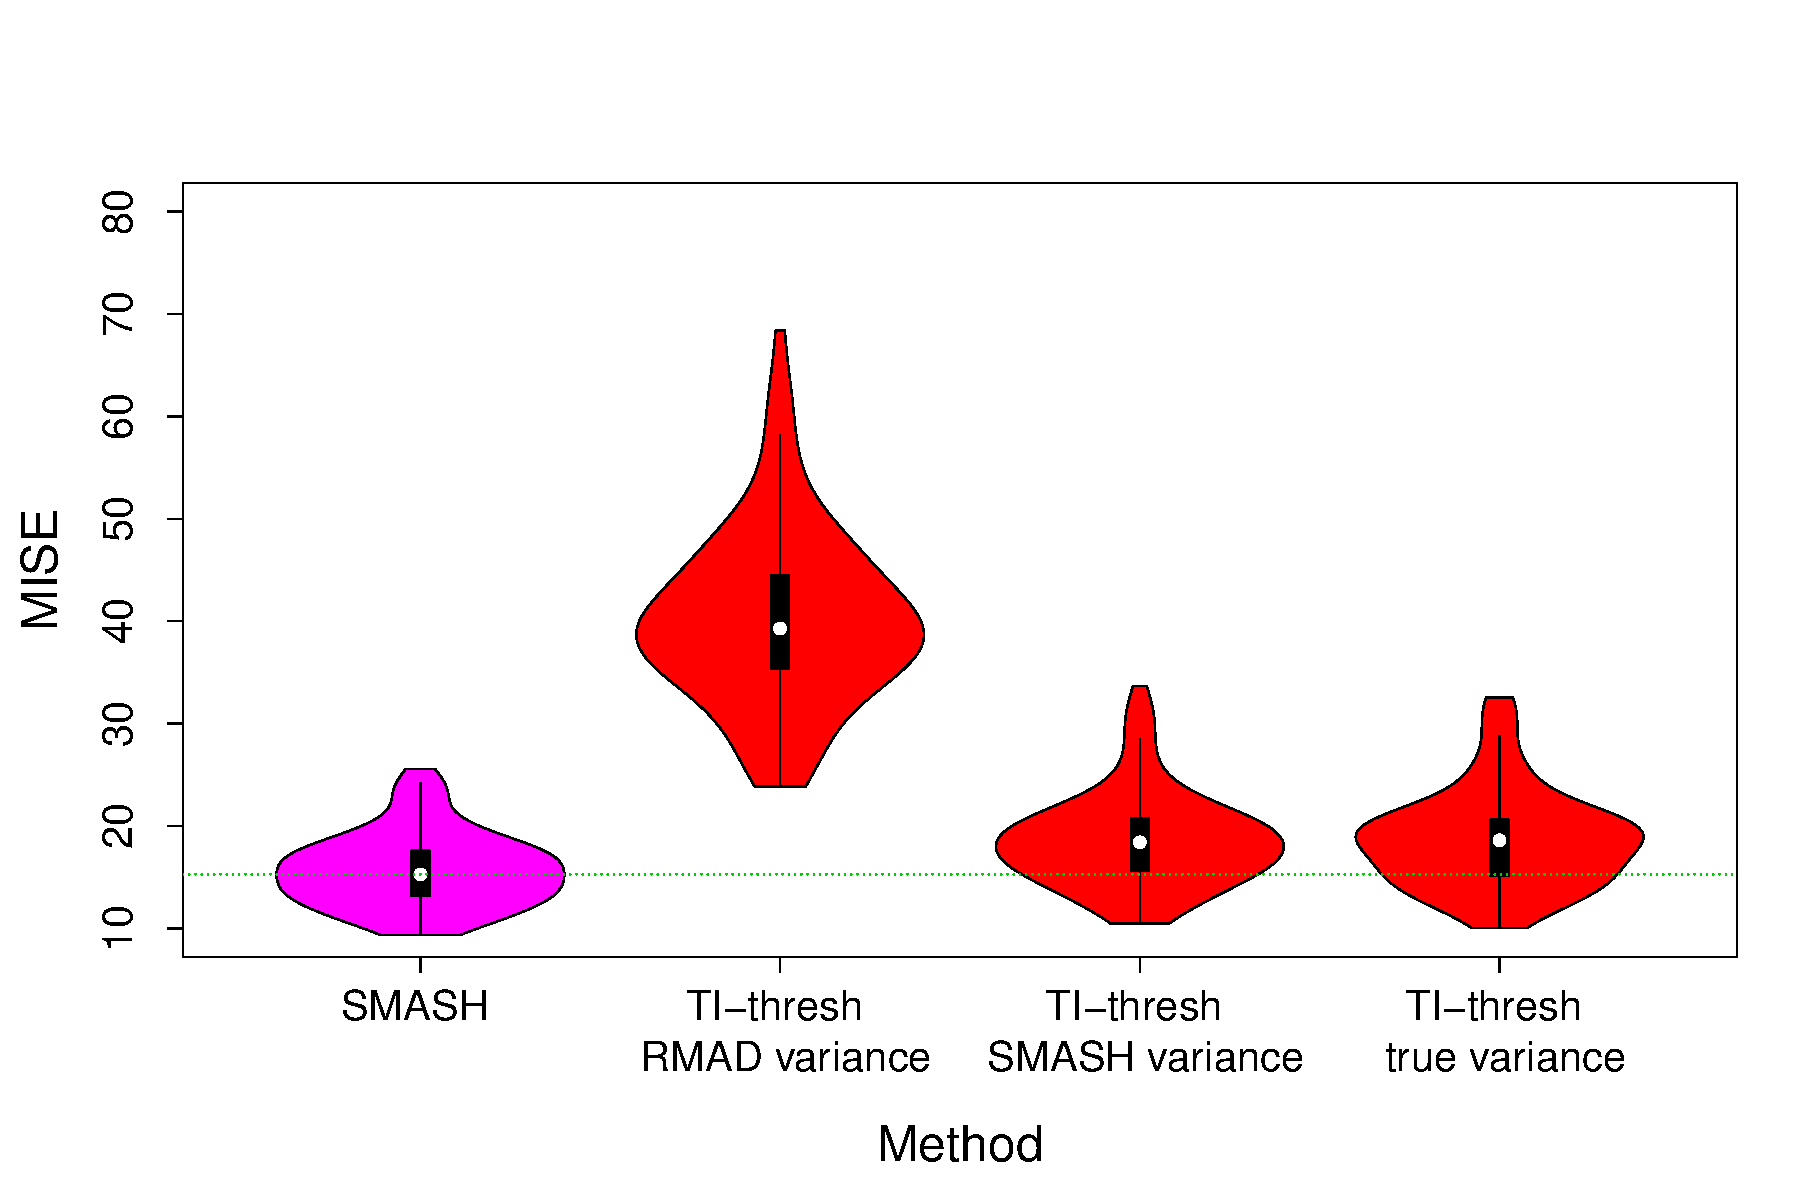
\includegraphics[width=\textwidth]{violin_gaus_hetero_ti.pdf}
        %\caption{}
        %\label{fig:gaus_hetero_ti}
    %\end{subfigure}
		%\hfill
    %\begin{subfigure}[b]{0.45\textwidth}
        %\centering
        %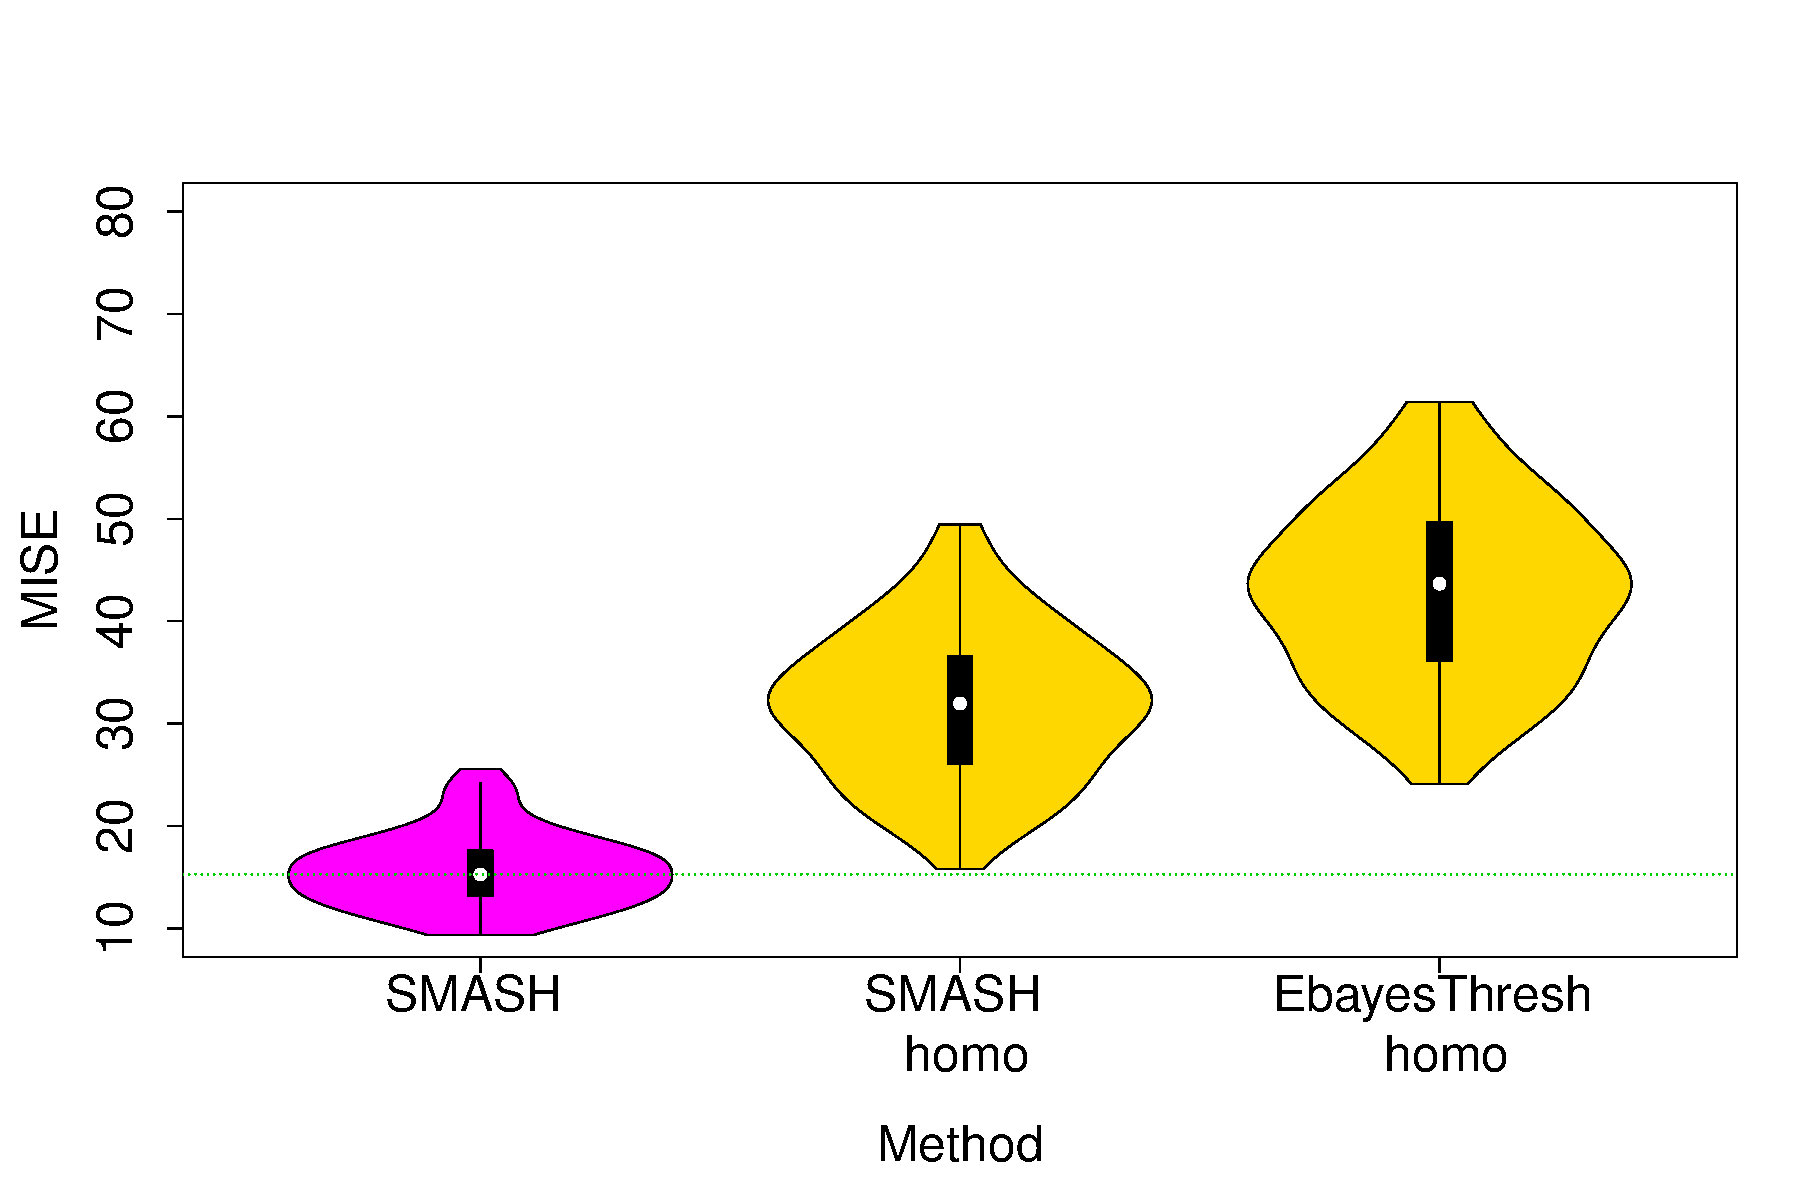
\includegraphics[width=\textwidth]{violin_gaus_hetero_homo.pdf}
        %\caption{}
        %\label{fig:gaus_hetero_homo}
    %\end{subfigure}
		%\hfill
    %\begin{subfigure}[b]{0.45\textwidth}
        %\centering
        %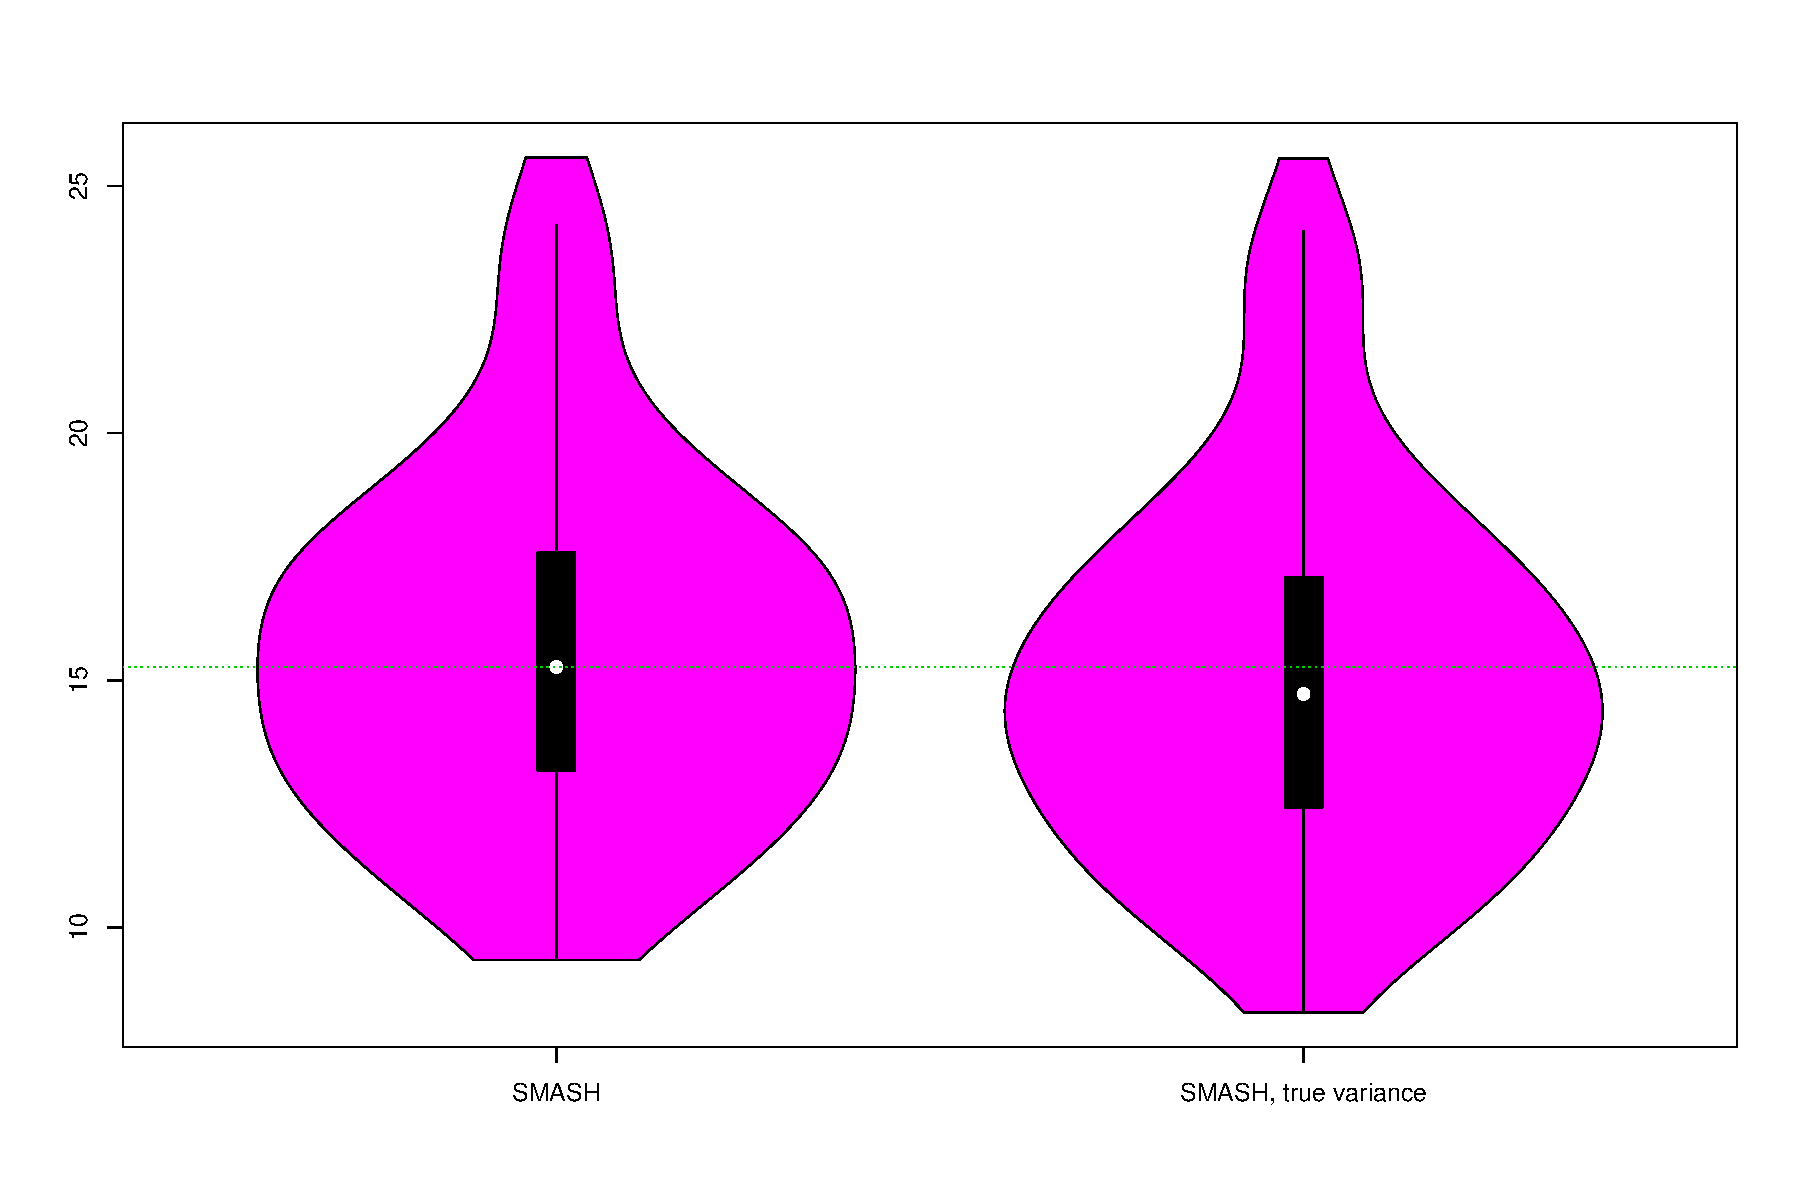
\includegraphics[width=\textwidth]{violin_gaus_hetero_smash.pdf}
        %\caption{}
        %\label{fig:gaus_hetero_smash}
    %\end{subfigure}
    %\caption{Violin plots of MISEs for various methods. Dashed green line indicates the median MISE for SMASH. a) compares SMASH against TI-thresh with variance estimated by RMAD, variance estimated by SMASH, and the true variance. b) demonstrates the importance of taking heteroskedasticity into account, and c) reveals the performance gain of SMASH when it is provided the true variance.}
    %\label{fig:gaus_hetero}
%\end{figure}

\begin{figure}[ht]
\centering
    \begin{subfigure}[b]{0.45\textwidth}
        \centering
        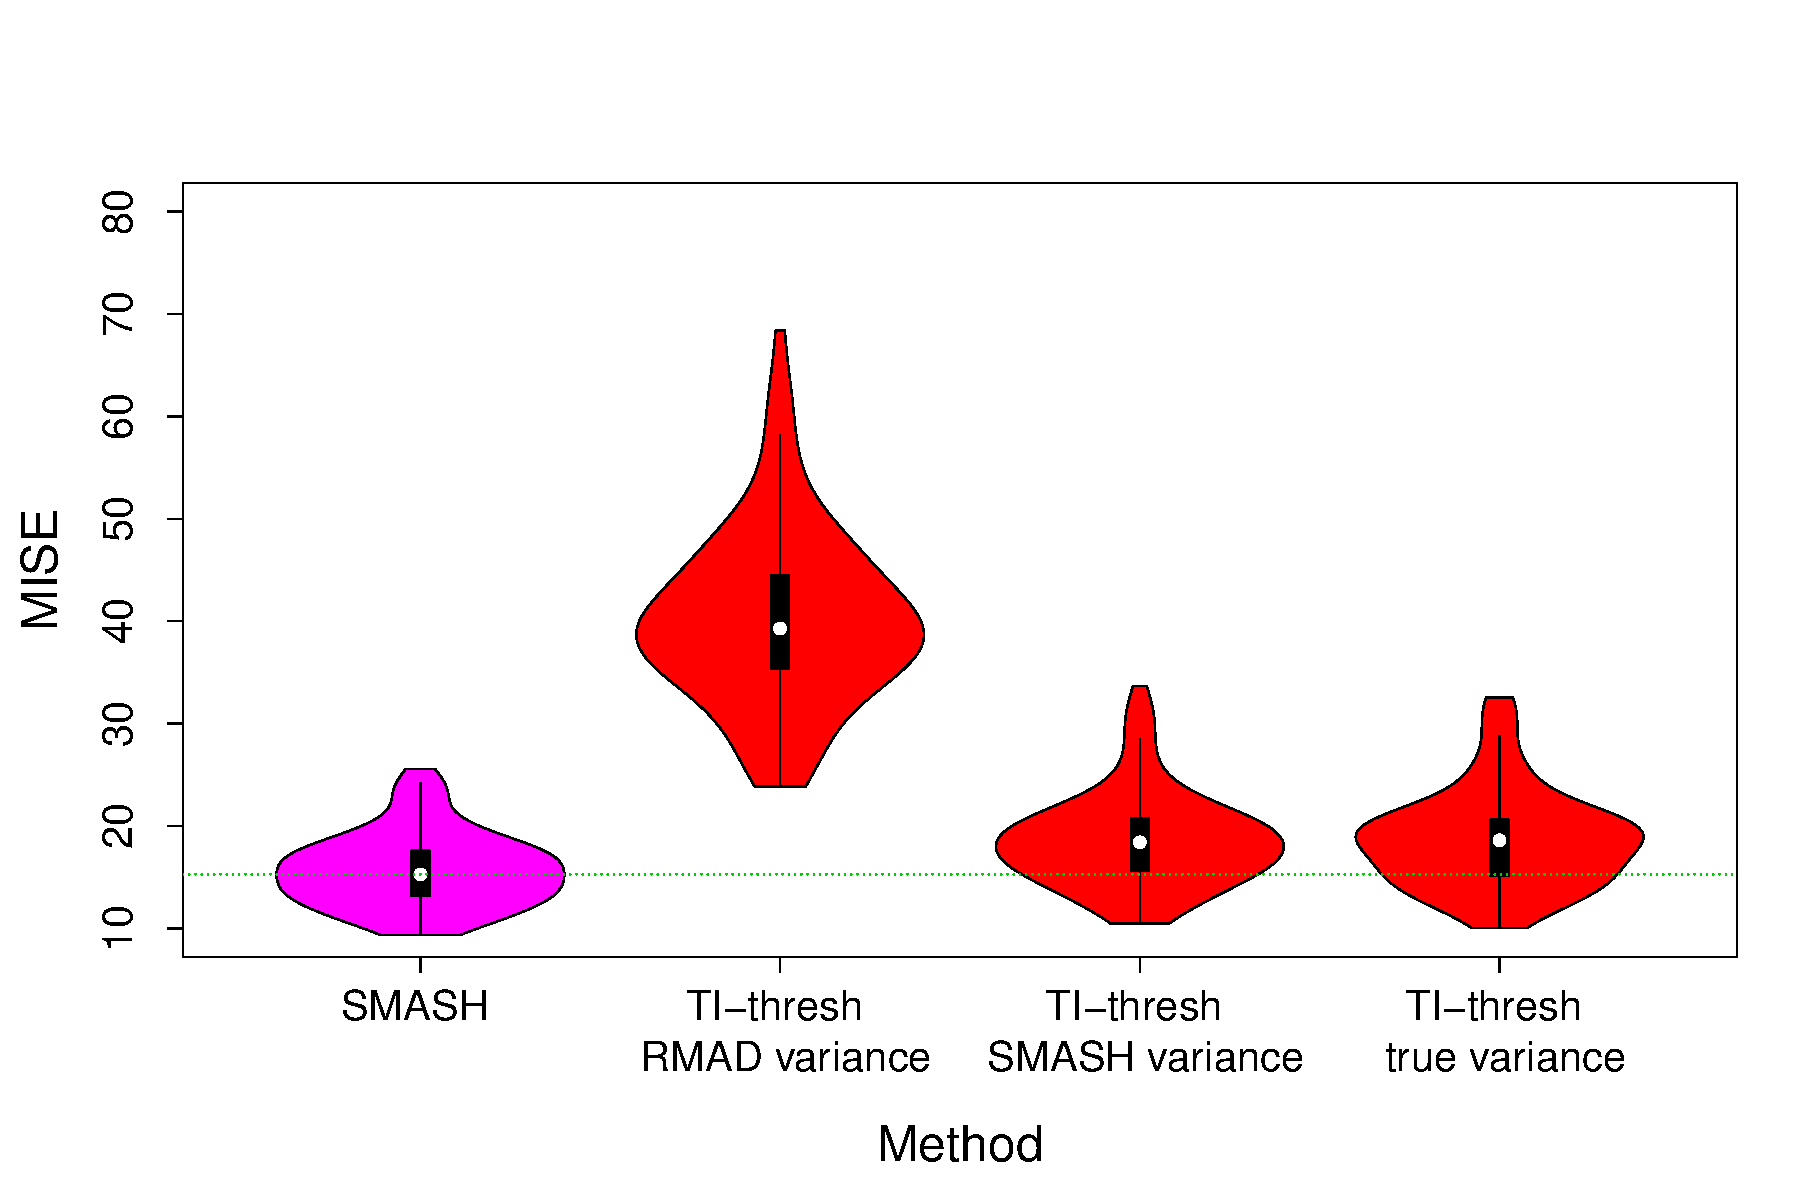
\includegraphics[width=\textwidth]{violin_gaus_hetero_ti.pdf}
        \caption{}
        \label{fig:gaus_hetero_ti}
    \end{subfigure}
		\hfill
    \begin{subfigure}[b]{0.45\textwidth}
        \centering
        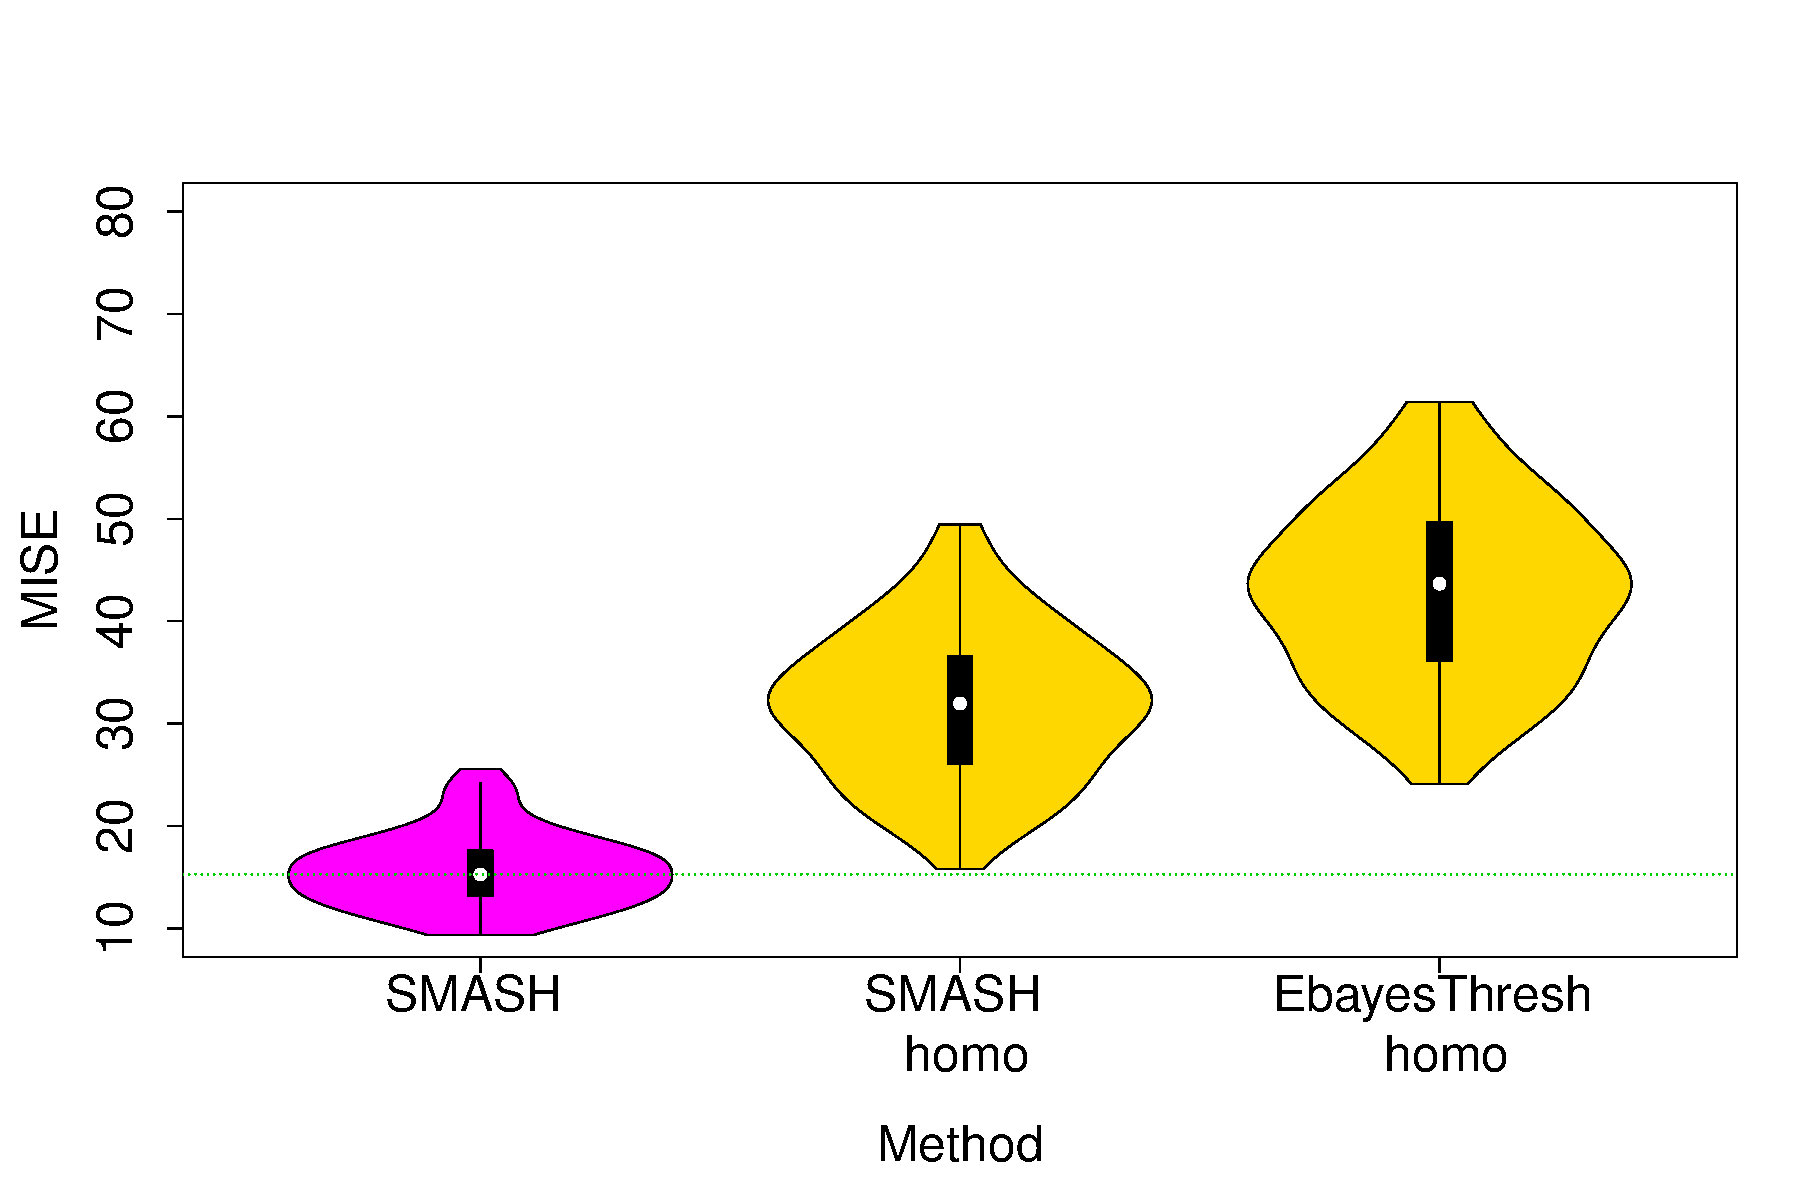
\includegraphics[width=\textwidth]{violin_gaus_hetero_homo.pdf}
        \caption{}
        \label{fig:gaus_hetero_homo}
    \end{subfigure}
		\hfill
    \begin{subfigure}[b]{0.45\textwidth}
        \centering
        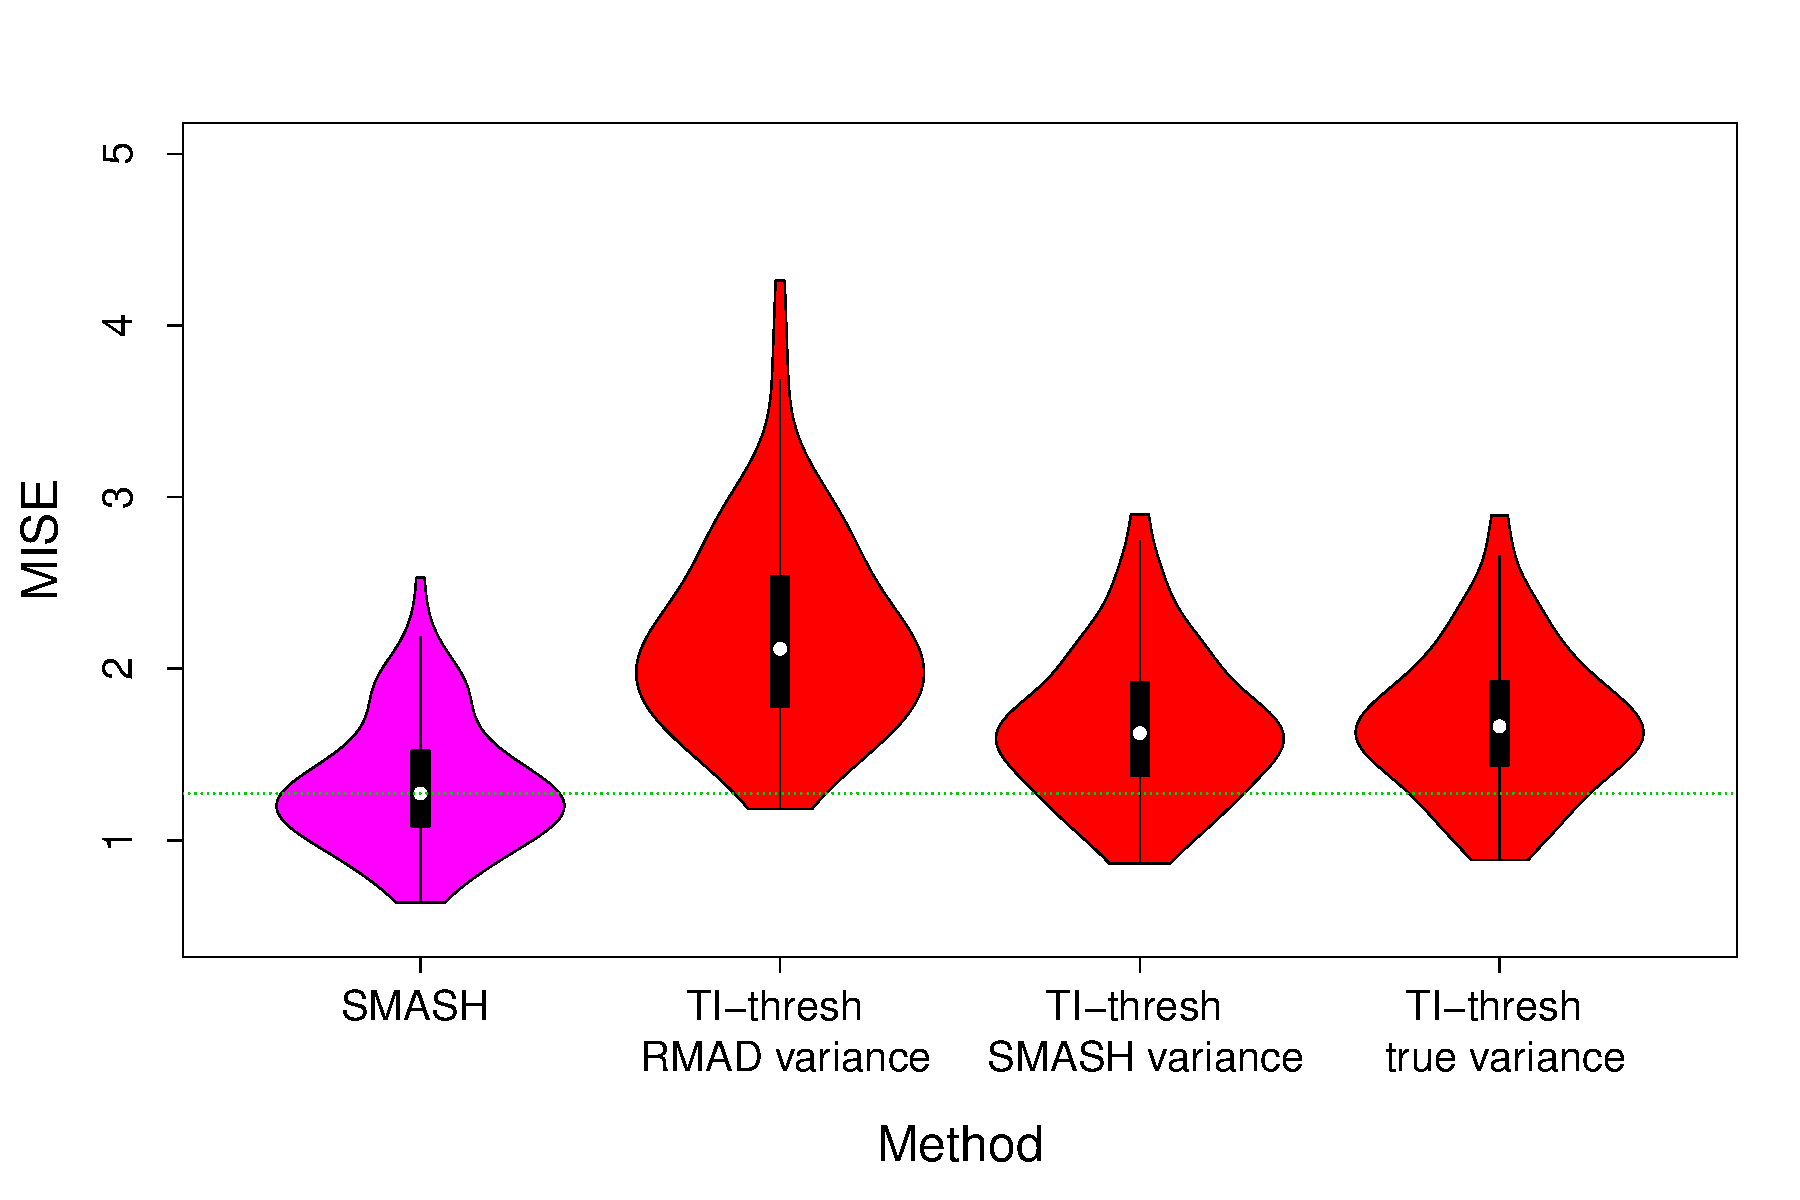
\includegraphics[width=\textwidth]{violin_gaus_hetero_ti_2.pdf}
        \caption{}
        \label{fig:gaus_hetero_smash}
    \end{subfigure}
		\hfill
    \begin{subfigure}[b]{0.45\textwidth}
        \centering
        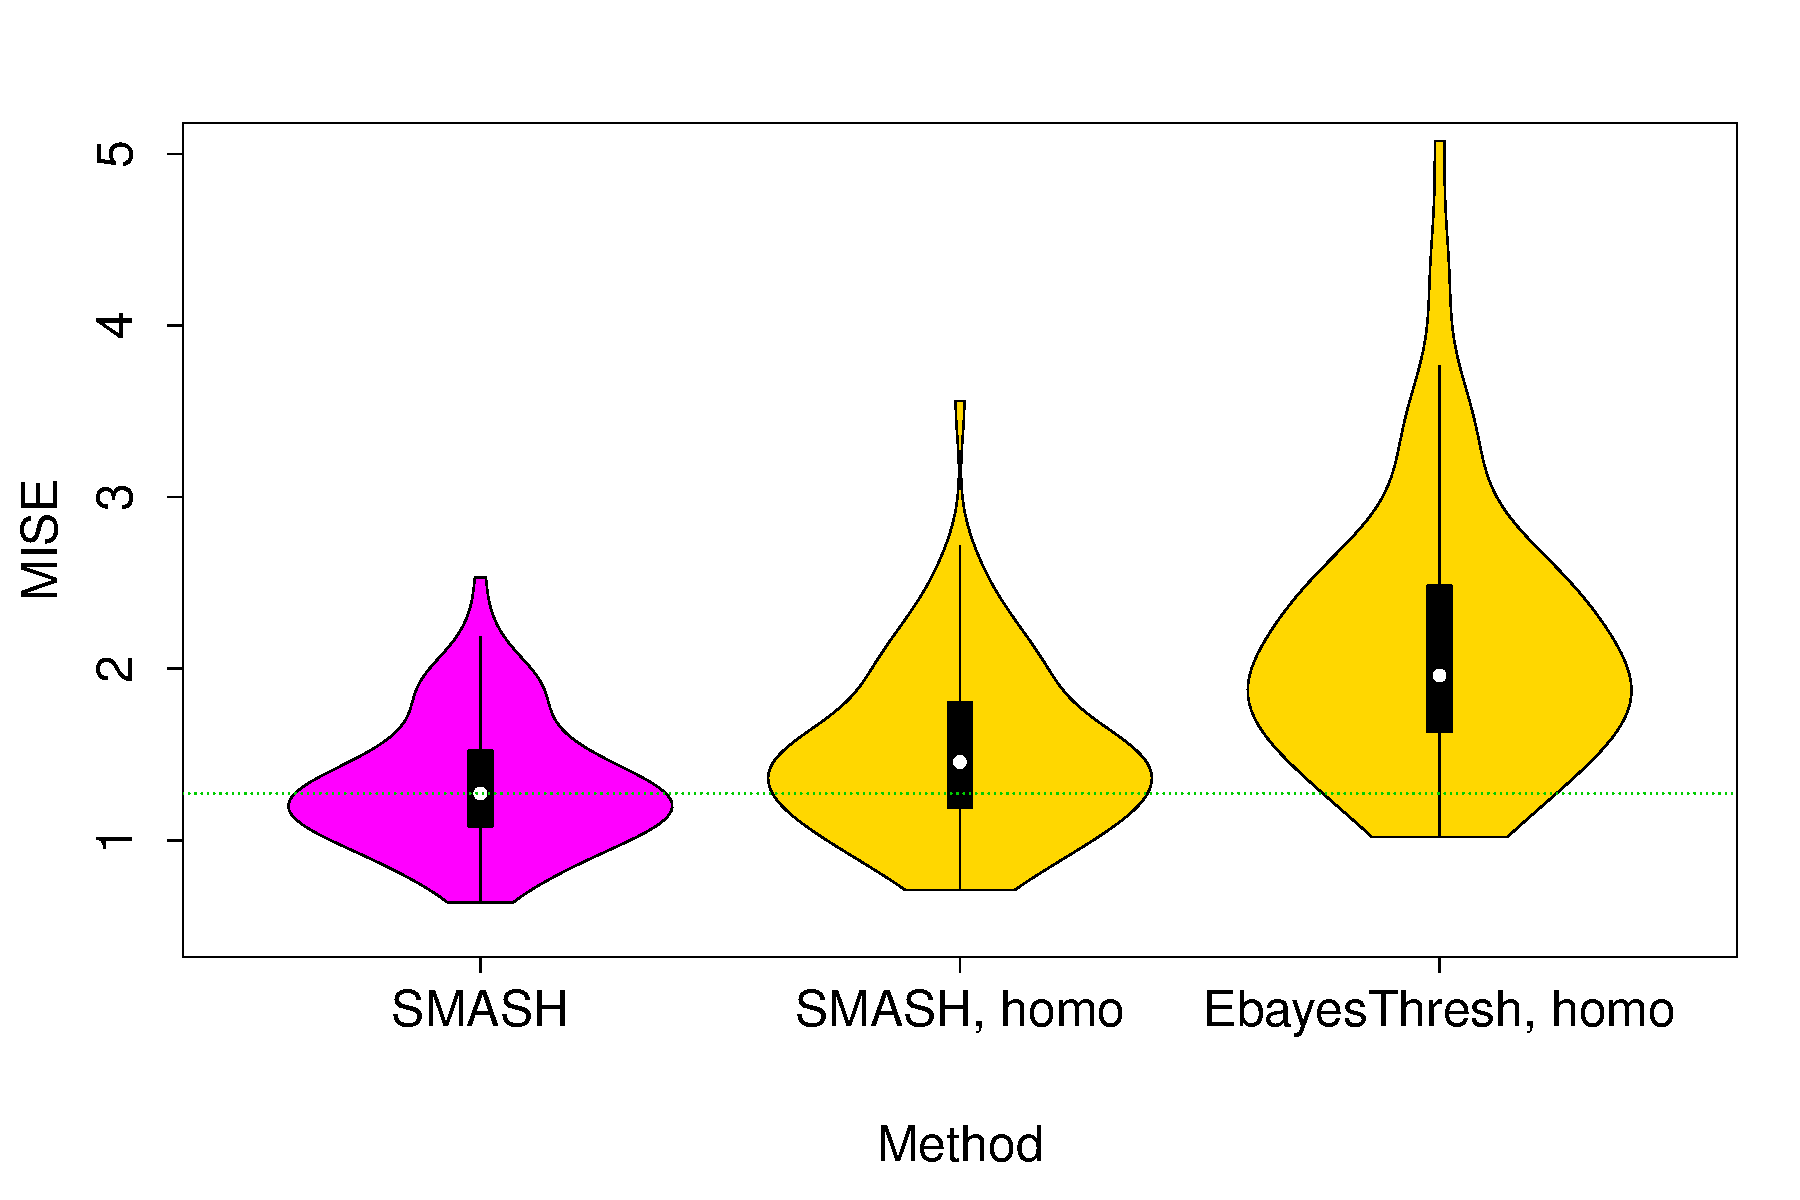
\includegraphics[width=\textwidth]{violin_gaus_hetero_homo_2.pdf}
        \caption{}
        \label{fig:gaus_hetero_smash}
    \end{subfigure}
    \caption{Violin plots of MISEs for various methods. Dashed green line indicates the median MISE for SMASH. a) compares SMASH against TI-thresh with variance estimated by RMAD, variance estimated by SMASH, and the true variance. b) demonstrates the importance of taking heteroskedasticity into account, and c) reveals the performance gain of SMASH when it is provided the true variance.}
    \label{fig:gaus_hetero}
\end{figure}



Several facts are immediately clear from figure \ref{fig:gaus_hetero}: 
\begin{enumerate}
\item From \ref{fig:gaus_hetero_ti}: SMASH does better than all TI-thresh variants, including the case when the true variance is provided, demonstrating the excellent finite sample performance of SMASH.
\item From \ref{fig:gaus_hetero_ti}: using the variance estimate from SMASH as an input to TI-thresh improves the accuracy of TI-thresh substantially, compared with using RMAD to estimate the variance as in Gao (1997)
\item From \ref{fig:gaus_hetero_homo}: accounting for heteroskedasticity allows SMASH to vastly outperform methods which assume homoskedastic errors.
\item From \ref{fig:gaus_hetero_homo}: empirical Bayes methods are more robust to violations of homoskedasticity compared with TI-thresholding.
\item From \ref{fig:gaus_hetero_smash}: Providing the true variance to SMASH does not substantially improve the performance of the methods compared to the case when SMASH estimates its own variance function. Hence, we can reasonably assume that SMASH does a good job of variance estimation, although this claim relies heavily on the variance function at hand. For example, the Bumps variance function (see appendix ?) is extremely difficult to estimate, and SMASH will perform much better when provided with the true variance function.
\end{enumerate}

Since our method also provides variance estimates, one could potentially perform similar assessments for different variance functions as with mean functions. In this particular study, we compare our method against the only joint mean and variance estimation procedure for which software is easily available. Specifically, we consider the Mean Field Variational Bayes (MFVB) methodology developed by Menictas \& Wand (2014) for heteroskedastic Gaussian regression. Since MFVB is splines-based (and hence less adaptive locally), we chose the smooth mean and standard deviation functions (A) from Menictas \& Wand (2014) as our test functions, plotted in Figure \ref{fig:mfvb_fn} and denoted by $m(\cdot)$ and $sd(\cdot)$ respectively. We then considered two different simulation scenarios:
\begin{enumerate}
\item $n=500$ independent $(X_i,Y_i)$ pairs were generated. The $X_i$'s were distributed as Uniform(0,1), and the $Y_i$'s were distributed as $N(m(x_i),sd(x_i))$. The performance of a given method is measured by the standard MSE evaluated at 201 equally spaced points on $(X_{min},X_{max})$ for both the mean and the standard deviation functions.
\item $n=1024$ independent $(X_i,Y_i)$ pairs were generated. The $X_i$'s were deterministic and equally spaced on (0,1), while the $Y_i$'s were distributed as $N(m(x_i),sd(x_i))$. The performance of a given method is measured by the MSE evaluated at the 1024 $X_i$'s for both the mean and the standard deviation functions.
\end{enumerate}
\begin{figure}[ht]
\centering
    \begin{subfigure}[b]{0.45\textwidth}
        \centering
        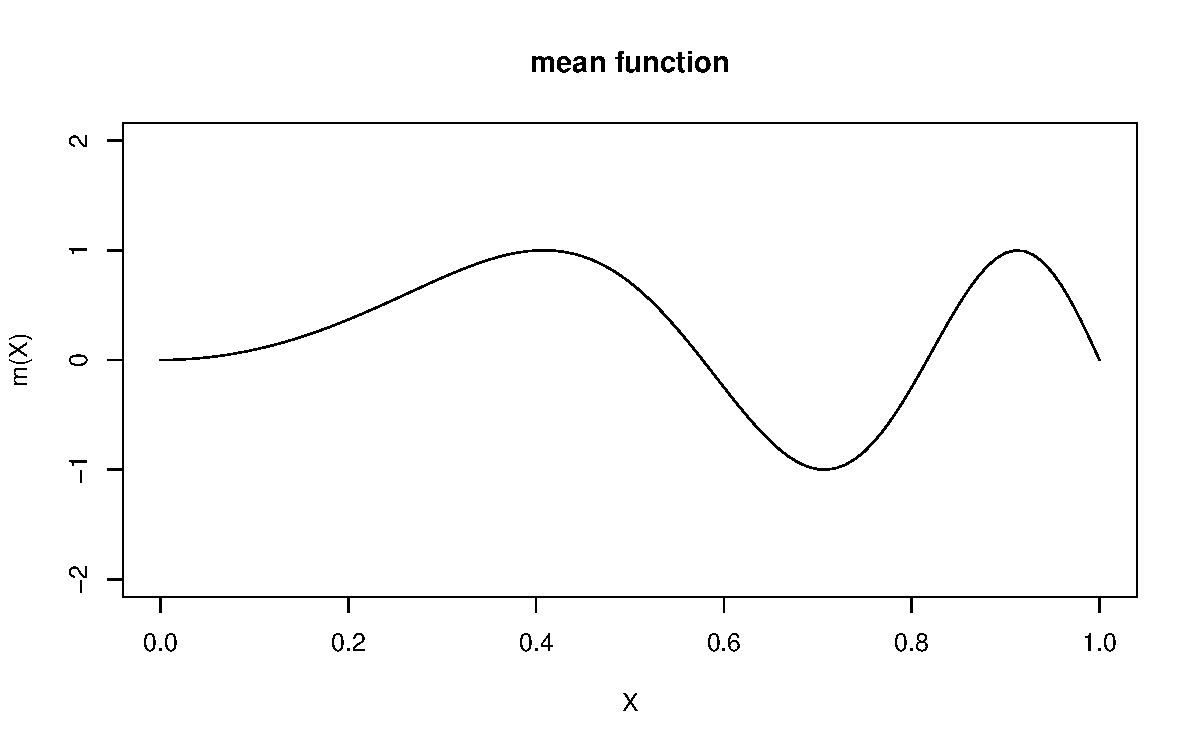
\includegraphics[width=\textwidth]{mfvb_mean.pdf}
        \caption{}
        \label{fig:mfvb_mean}
    \end{subfigure}
    \hfill
    \begin{subfigure}[b]{0.45\textwidth}
        \centering
        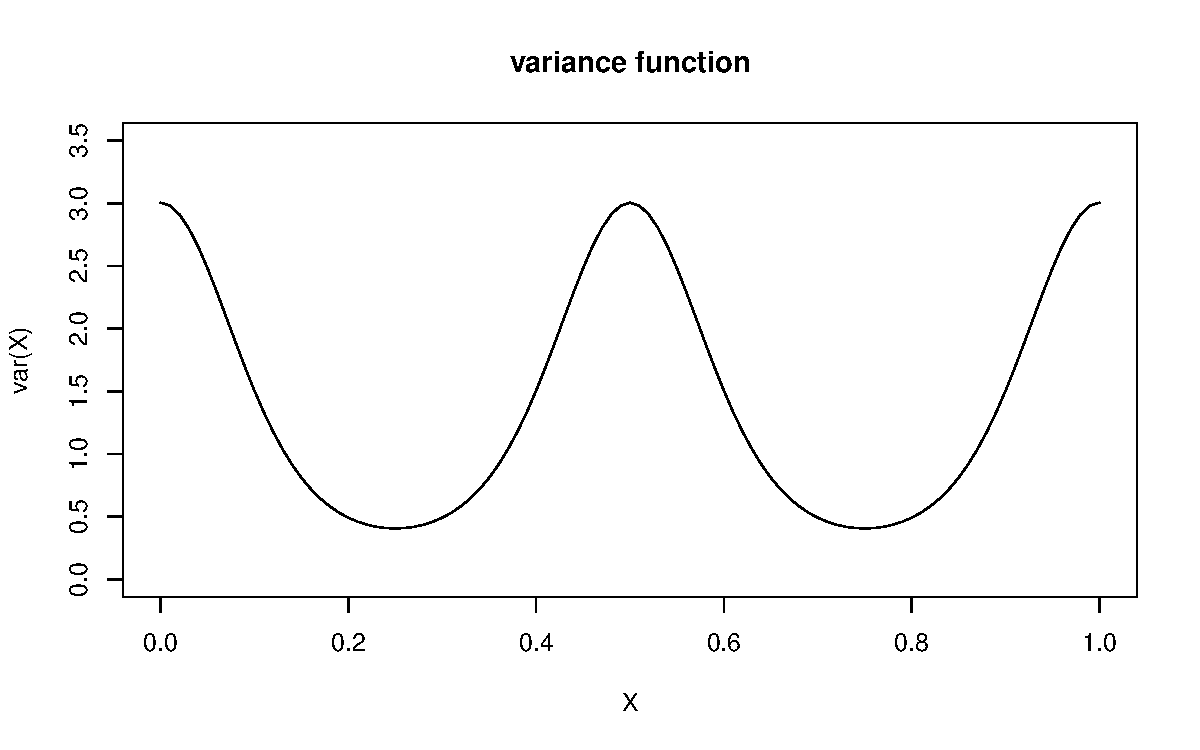
\includegraphics[width=\textwidth]{mfvb_var.pdf}
        \caption{}
        \label{fig:mfvb_var}
    \end{subfigure}
    \caption{Mean (a) and variance (b) functions used in the simulation study comparing SMASH against MFVB.}
    \label{fig:mfvb_fn}
\end{figure}
In the first scenario, the number of data points is not a power of two, nor are the point equally spaced. To deal with these complications, we adapted and modified the standard symmetric extension procedure commonly used in wavelet settings. We first mirrored the data about the right edge and extract the first $2^{\lfloor\log_2(2n)\rfloor}$ sample points. This ensures that the number of data points in the new ``dataset'' is a power of two, and the mean curve would be continuous at the right edge. To further ensure that the input to the Gaussian denoising method is periodic, we then reflected the new dataset about the right edge and used this as the final input. To obtain the original mean and variance functions, we extracted the first $n$ points from the outputs (mean and variance) of our denoising technique. Since the data points are not evenly spaced, we took the simplest approach and applied our method treating the observations as if they were evenly spaced. This approach is not only intuitively appealing, but can also be considered a formal treatment of unequally spaced data in traditional wavelet settings (see Sardy et al. (1999)). Evaluation of MSE at the 201 equally spaced points is then based on simple linear interpolation between the estimated points. Tables \ref{table:mfvb_comp} display the MSEs over 100 independent runs for each scenario.
\begin{table}[ht]
\centering
\begin{tabular}{rrrrr}
\hline
& \multicolumn{2}{c}{Scenario 1}&\multicolumn{2}{c}{Scenario 2}\\
\cline{2-5}
& mean & sd & mean & sd \\
\hline
MFVB & 0.0330 & 0.0199 & 0.0172 & 0.0085 \\
SMASH & 0.0334 & 0.0187 & 0.0158 & 0.0065 \\
\hline
\end{tabular}
\caption{MSEs of MFVB and SMASH for two simulation scenarios}
\label{table:mfvb_comp}
\end{table}

Note that wavelets in general are poorly suited for dealing with the setup in Scenario 1; not only are the number of data points not a power of two, they are also not equally spaced. Also, linear interpolation between sample points was used in computing the MSE, further impacting the accuracy of SMASH. At the same time, spline-based methods such as MFVB are well suited to dealing with smooth mean and variance functions such as those used in the simulations, whereas wavelet methods can better deal with spatial inhomogeneity which are present in functions such as those presented in Figure \ref{fig:gaus_homo}. Despite all these limitations, our method performs comparably to MFVB in terms of mean estimation for the simulation scheme presented in Scenario 1, and has a lower MSE in terms of variance estimation. For Scenario 2, our method outperforms MFVB in both mean and variance estimation. 

Thus far, we have demonstrated that our method does a good job of mean and variance estimation for a variety of situations in the Gaussian case. As such, we now turn our attention to the Poisson case. For this simulation study, we considered different test functions and Poisson intensities for a given sample size of $n=1024$ as in Timmermann \& Nowak (1999) and Fryzlewicz \& Nason (2004), over 100 independent runs. Figure \ref{fig:pois_sim} compares the MISE of SMASH with Haar-Fisz (Fryzlewicz \& Nason (2004)) and BMSM (Kolaczyk (1999b)), which are two popular and accurate Poisson denoising techniques, for the ``Bursts'' function with (min,max) intensities of (0.01,3) and (1/8,8), which are of primary interest. Complete results, including a (min,max) intensity of (1/128, 128), are included in appendix \textcolor{red}{where?}. From figure \ref{fig:pois_sim}, it is clear that SMASH outperforms both methods, and the claim holds true in general. As an exception, Haar-Fisz outperforms both SMASH and BMSM for certain test functions with a (min,max) intensity of (1/128,128) when the asmyptotic variance of 1 is assumed in the Gaussian wavelet thresholding stage of the Haar-Fisz algorithm, but underperforms when the variance is estimated from the data instead. Besides the assumption of unit variance, the inconsistent performance of Haar-Fisz could also be attributed to the choice of the primary resolution level used, which can substantially affect the performance of Haar-Fisz. Here we analyzed primary resolution levels of 4, 5, 6 and 7. On the other hand, SMASH outperforms BMSM consistently, even though our method is based on the same likelihood factorization used in the latter. We can thus conclude that the choice of ASH as the shrinkage procedure (with the necessary likelihood approximations) is superior to that used in BMSM. As will be discussed later, using the formulation in SMASH also makes it easily extensible to multiple samples in the context of a (generalized) linear model.
\begin{figure}
\centering
    \begin{subfigure}[b]{0.45\textwidth}
        \centering
        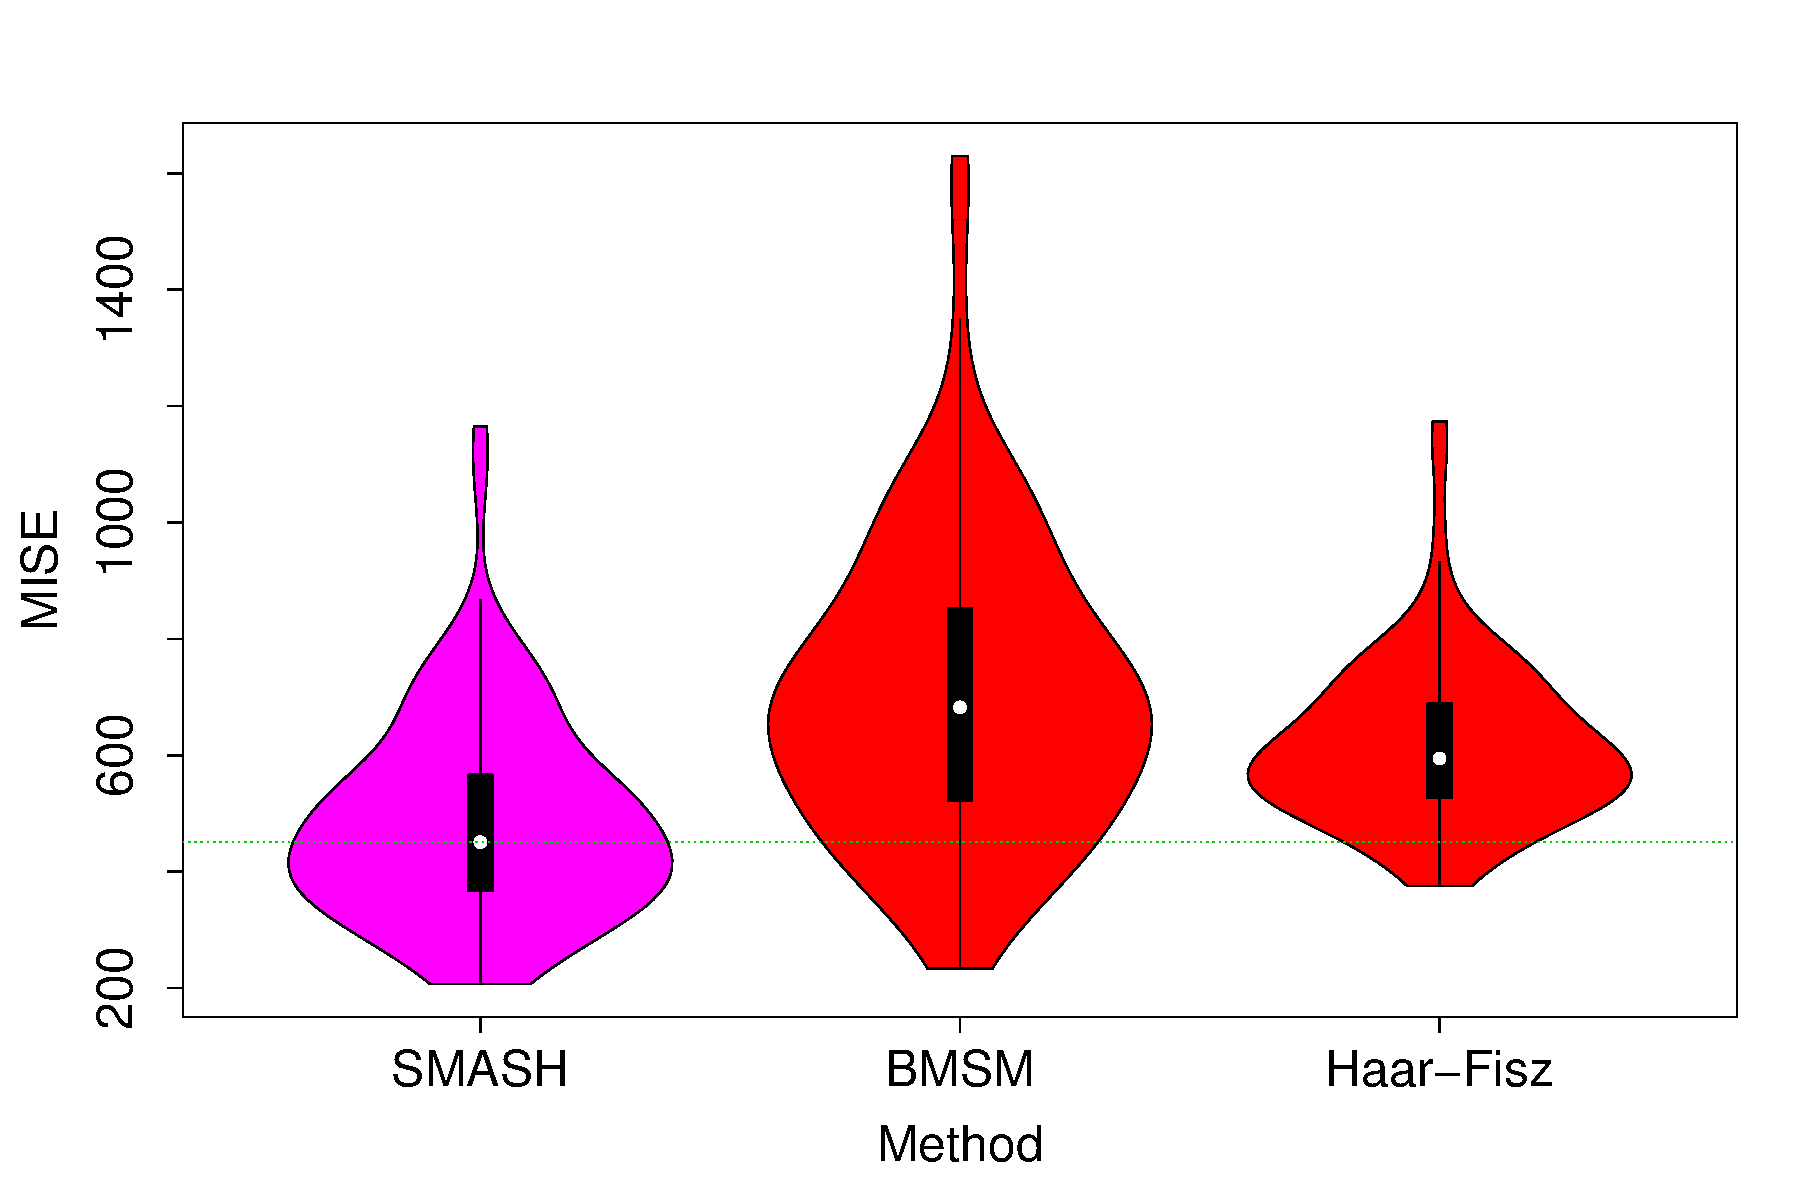
\includegraphics[width=\textwidth]{violin_pois_1.pdf}
        \caption{}
        \label{fig:pois_1}
    \end{subfigure}
		\hfill
    \begin{subfigure}[b]{0.45\textwidth}
        \centering
        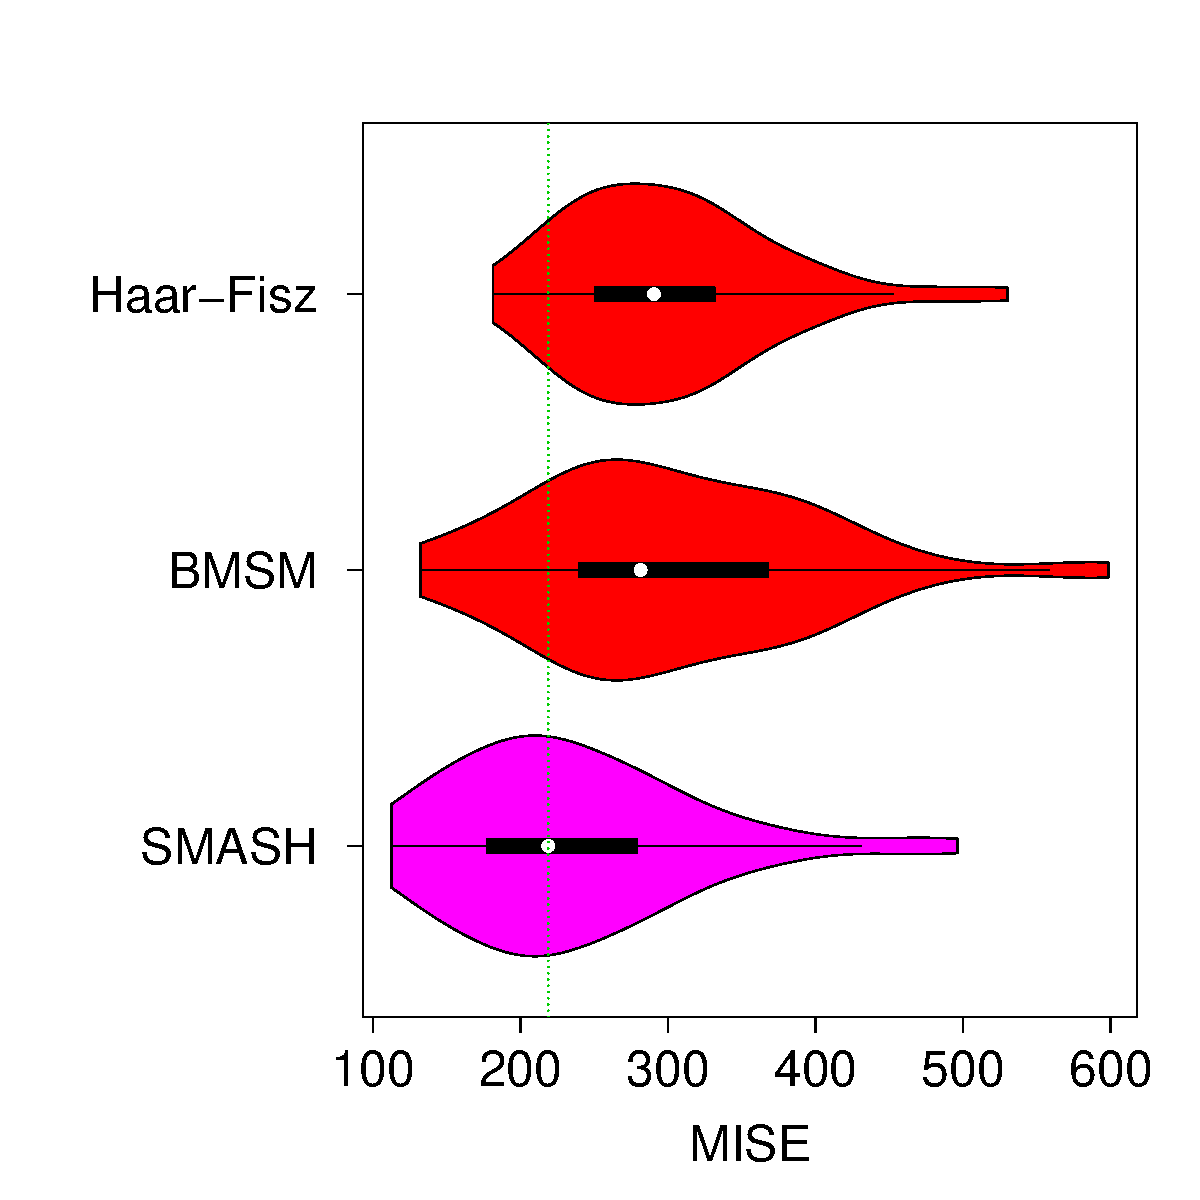
\includegraphics[width=\textwidth]{violin_pois_8.pdf}
        \caption{}
        \label{fig:pois_8}
    \end{subfigure}
    \caption{Violin plots of MISEs for various methods. a) corresponds to a (min,max) intensity of (0.01,3), and b) corresponds to a (min,max) intensity of (1/8,8)}
    \label{fig:pois_sim}
\end{figure}

In terms of computation, we note that SMASH is much more efficient than Haar-Fisz with external cyclespinning, as the latter method needs to be rerun for each shift of the data. However, a direct comparison between SMASH and BMSM is uninformative, as they are coded in different programming environments. Nevertheless, the similarities between the two methods imply that they should behave identically in this aspect, barring differences in coding.

Overall, these simulation studies demonstrate the ability of our method to accurately recover the mean functions for both the Gaussian and Poisson cases, and highlight the flexibility and adaptiveness of the shrinkage procedure ASH. Although we have considered an extensive range of scenarios here, including different SNRs, sample sizes, variance functions, test functions and mean intensities where applicable, the performance of our method on real data has yet to be determined. In the next section, we will apply our method to two example datasets that have been discussed in previous work, and comment on the resulting estimates.



\section{Application to real datasets}
\subsection{Three-month Treasury Bill Yields}
In this section we apply the Gaussian and Poisson denoising techniques to one example dataset each. For the Gaussian case, we looked at yields of secondary market rates from three-month Treasure bills, which were recorded weekly on Fridays. These rates were quoted on a discount basis and annualized using a 360-day year of bank interest. To match the analysis in Fan \& Yao (1998), we used 1735 weekly observations spanning Jan. 5 1962 to Mar. 31 1995. The data are plotted in Figure \ref{fig:tb_raw_data}. Similar to Fan \& Yao (1998), we fit an autoregressive model of order 5 (AR(5)) to the data and obtained the following:
\begin{eqnarray}
T_t=1.228T_{t-1}-0.234T_{t-2}+0.028T_{t-3}+0.039T_{t-4}-0.066T_{t-5}+Y_t
\end{eqnarray}
where $T_t, t=1,...,1735$ is the time series for the yields, and $Y_t$ are the residuals from fitting the model. Figure \ref{fig:tb_res} shows the plot of $Y_t$ against $X_t\equiv T_{t-1}$. Our goal is to estimate the mean function defined by $E(Y_t|X_t=x)$ as well as the variance function $V(Y_t|X_t=x)$. Note that standard wavelet techniques are not designed for such types of data, where 1) repeated observations are present and 2) the number of data points is not a power of two and the points are unevenly spaced. To tackle the first issue, we use the median of the repeated observations at their respective sample points (see eg Delouille et al. (2004)). Next, we applied the procedure described in the Simulations section when comparing our method against MFVB, which was a modified version of symmetric extension. This deals with the second complication. The estimated mean and variance functions are given in Figures \ref{fig:tb_res} and \ref{fig:tb_var} respectively.

\begin{figure}
\centering
    \begin{subfigure}[b]{0.4\textwidth}
        \centering
        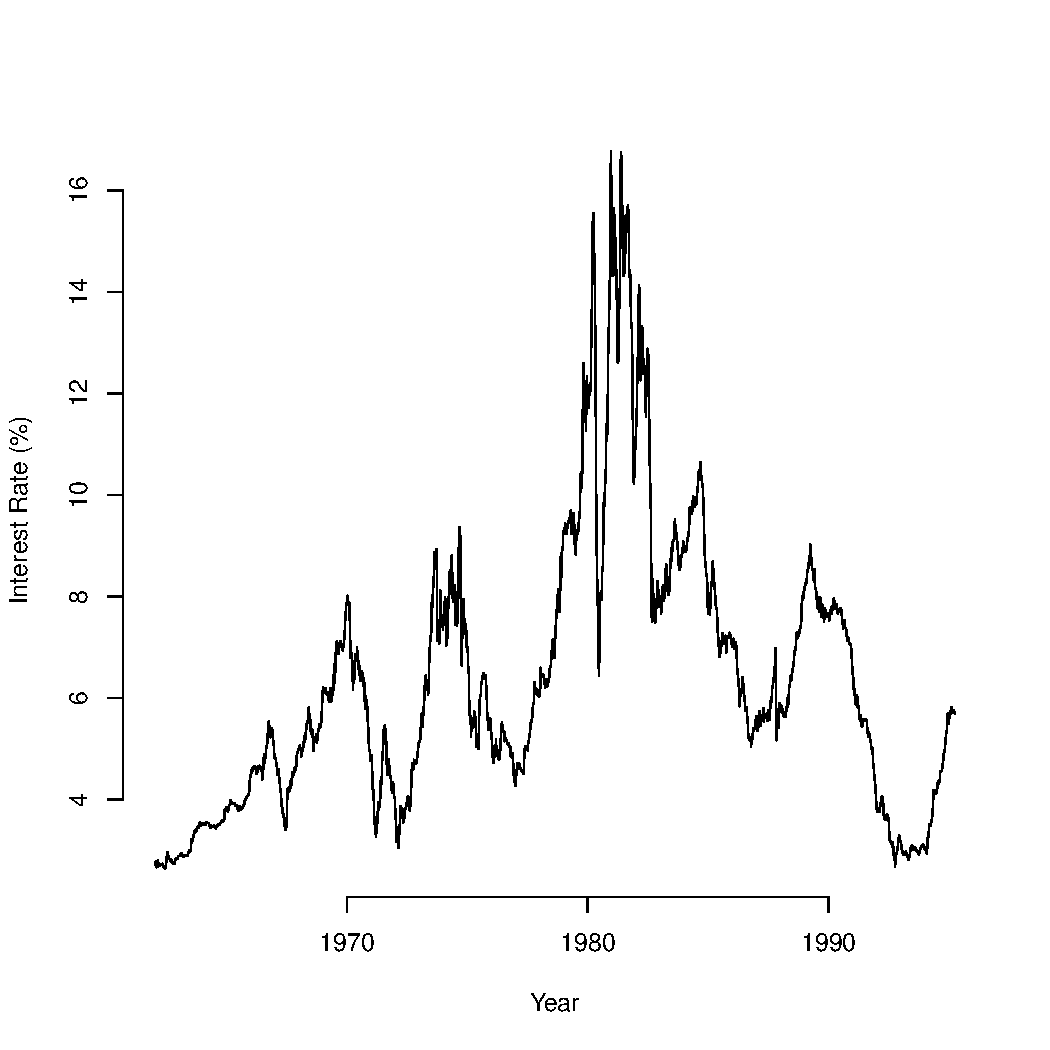
\includegraphics[width=\textwidth]{figures_treasury_a.pdf}
        \caption{}
        \label{fig:tb_raw_data}
    \end{subfigure}
    \hfill
    \begin{subfigure}[b]{0.4\textwidth}
        \centering
        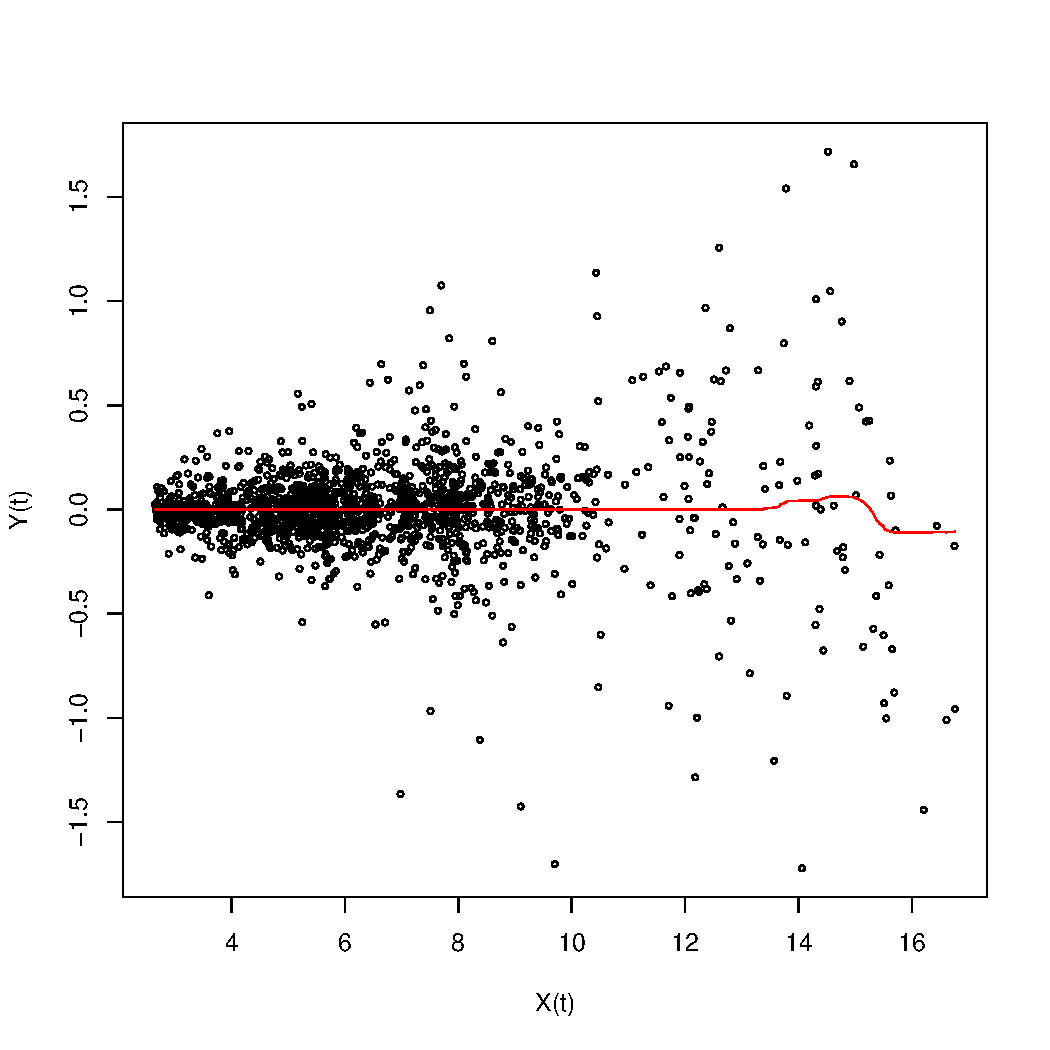
\includegraphics[width=\textwidth]{figures_treasury_b.pdf}
        \caption{}
        \label{fig:tb_res}
    \end{subfigure}
    \begin{subfigure}[b]{0.4\textwidth}
        \centering
        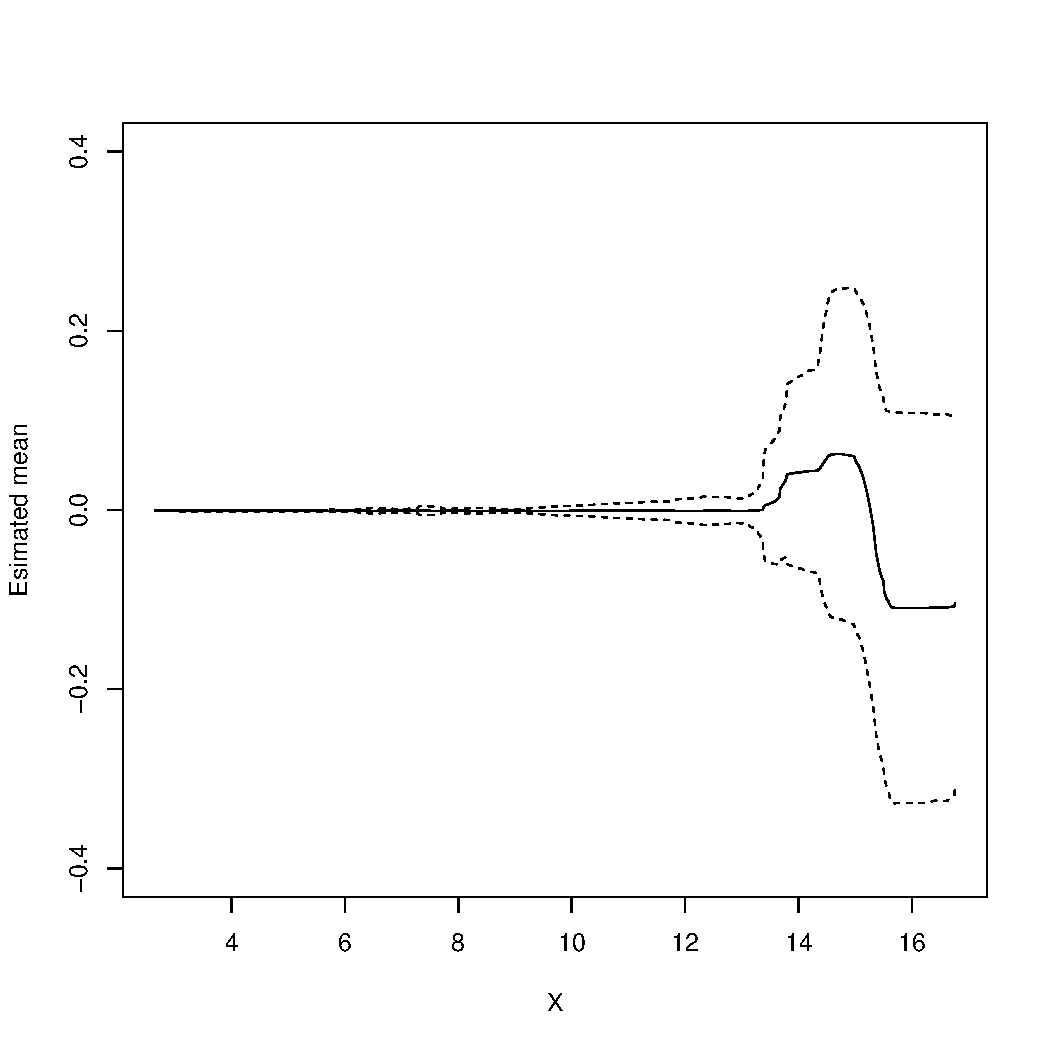
\includegraphics[width=\textwidth]{figures_treasury_c.pdf}
        \caption{}
        \label{fig:tb_mean}
    \end{subfigure}
    \hfill
    \begin{subfigure}[b]{0.4\textwidth}
        \centering
        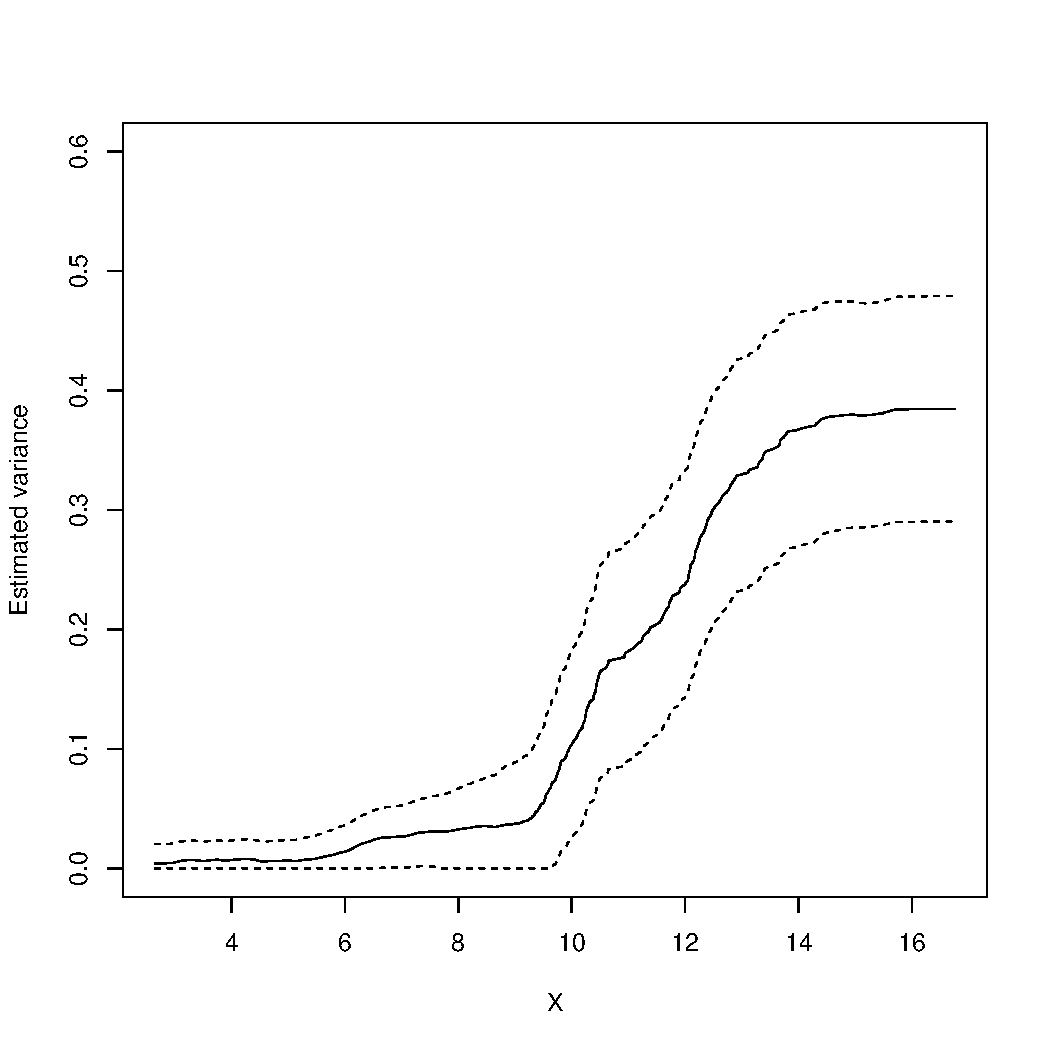
\includegraphics[width=\textwidth]{figures_treasury_d.pdf}
        \caption{}
        \label{fig:tb_var}
    \end{subfigure}
    \caption{Analysis of yields from three-month Treasury Bills. (a) Raw data of interest rates as a function of time. (b) Residuals $Y_t$ from fitting an AR(5) model to the data against $X_t\equiv T_{t-1}$. The red curve is the estimated mean curve from SMASH. (c) Plot of a zoomed-in version of the estimated mean curve, with approximate 95\% credible bands. (d) The estimated conditional variance curve, with approximate 95\% credible bands.}
\end{figure}

Except for possible boundary effects, our mean and conditional variance estimates are similar to those of Fan \& Yao (1998). Unfortunately, these boundary effects are difficult to deal with for non-periodic functions in the wavelet case, and our usage of symmetric extension with the Haar basis is just one possible solution. Better alternatives have been suggested by eg. Su et al. (2013), but is beyond the scope of discussion in this paper. Similar to the analysis in Fan \& Yao (1998), we found the correlation coefficient between the logarithm of $x_t$ and the logarithm $\hat{V}^{1/2}(Y_t|x_t)$ to be 0.949, which further supports the structural volatility model suggested by Andersen and Lund (source?):
\begin{eqnarray}
Var^{1/2}(Y_t|x_t)=\Ga x_t^{\Gb}
\end{eqnarray}
By performing least squares regression of $\log(\hat{V}^{1/2}(Y_t|x_t))$ on $\log(x_t)$, we have that $\hat{\Ga}=0.0106$ and $\hat{\Gb}=1.429$, which are similar to the values reported in Fan \& Yao (1998).
\newpage
\subsection{ChIP-Seq Data}
Here we apply our Poisson de-noising procedure to next generation sequencing data, commonly seen in the field of genomics. Specifically, we chose an example dataset from the ENCODE (\textbf{Enc}yclopedia \textbf{O}f \textbf{D}NA \textbf{E}lements) project launched by the National Human Genome Research Institute. This dataset contains reads from chromatin immunoprecipitation sequencing (ChIP-seq) measuring transcription factor binding in two different cell types, with two samples for each cell type. Due to the massive size of the data, we selected a representative portion of the reads of length $2^{15}$ from chromosome 1.
%Since we are looking mainly at univariate denoising here, we ran our method on each sample separately to produce the the plots in Figure \ref{fig:seq_smooth}.\\
%\begin{figure}[h]
%\centering
%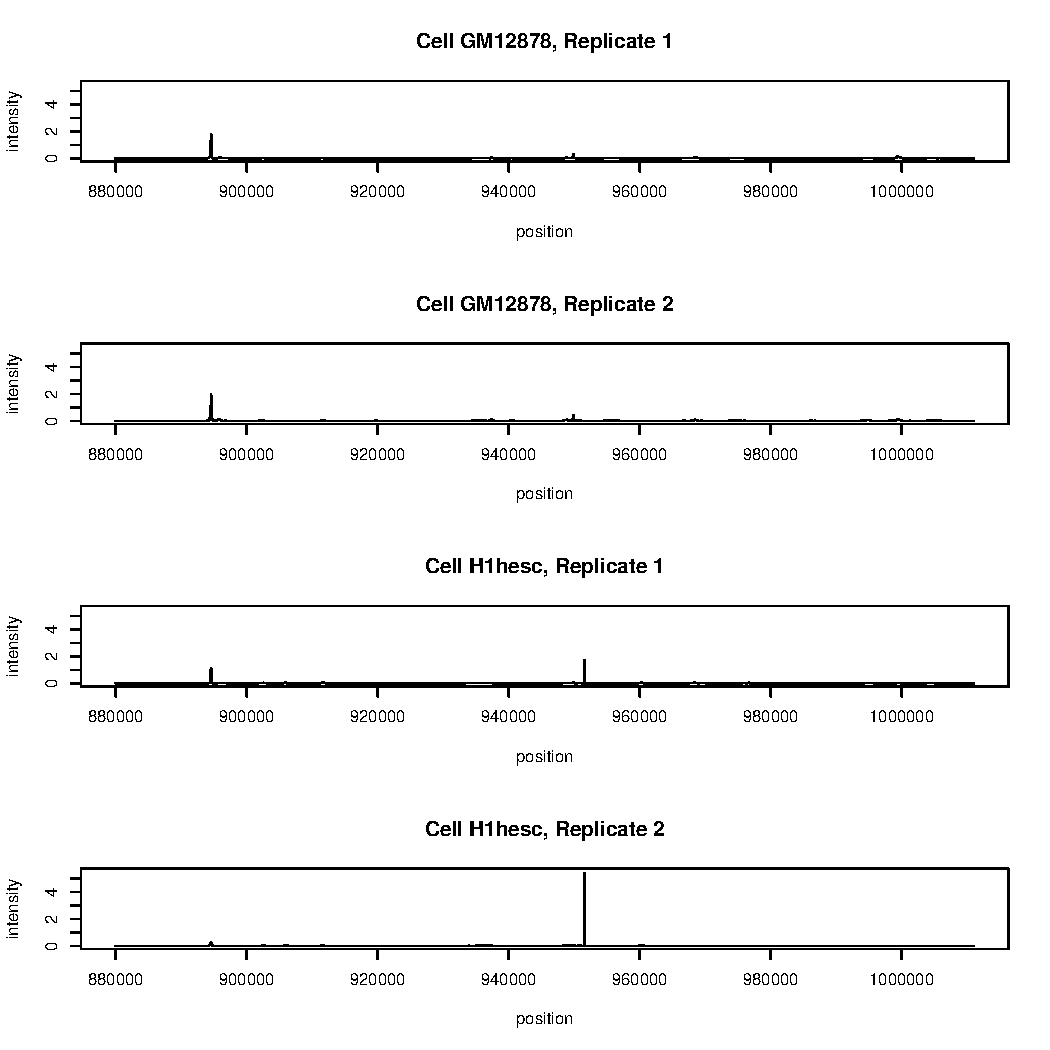
\includegraphics[scale=0.7]{smoothing_all.pdf}
%\caption{Estimated intensities from SMASH for 4 samples; the first two samples are two replicates from GM12878, a lymphoblastoid cell line, and the last two samples are two replicates from H1hesc, which are human embryonic stem cells. The reads are taken from position 880001 to 1011072 on chromosome 1.}
%\label{fig:seq_smooth}
%\end{figure}
%\bigskip
One goal of analyzing ChIP-seq data is to discover regions where transcription factors are likely to bind to DNA, thereby allowing us to better understand the mechanisms underlying gene regulation. These binding regions are often reflected in the data as ``peaks'', where more counts are present than background noise. Our method allows us to identify these peaks by looking at the estimated intensity function.
%In Figure \ref{fig:seq_smooth}, we immediately notice the presence of several large peaks around position 895000 for the first three samples, and around position 952000 for the last two samples.
To ensure that our method performs sensibly, we pooled the reads for the GM12878 cell line and ran our method as well as a popular peak calling procedure MACS on the selected region. The results are shown in Figure \ref{fig:seq_peak}.\\
\newpage
\begin{figure}
\centering
    \begin{subfigure}[b]{0.85\textwidth}
        \centering
        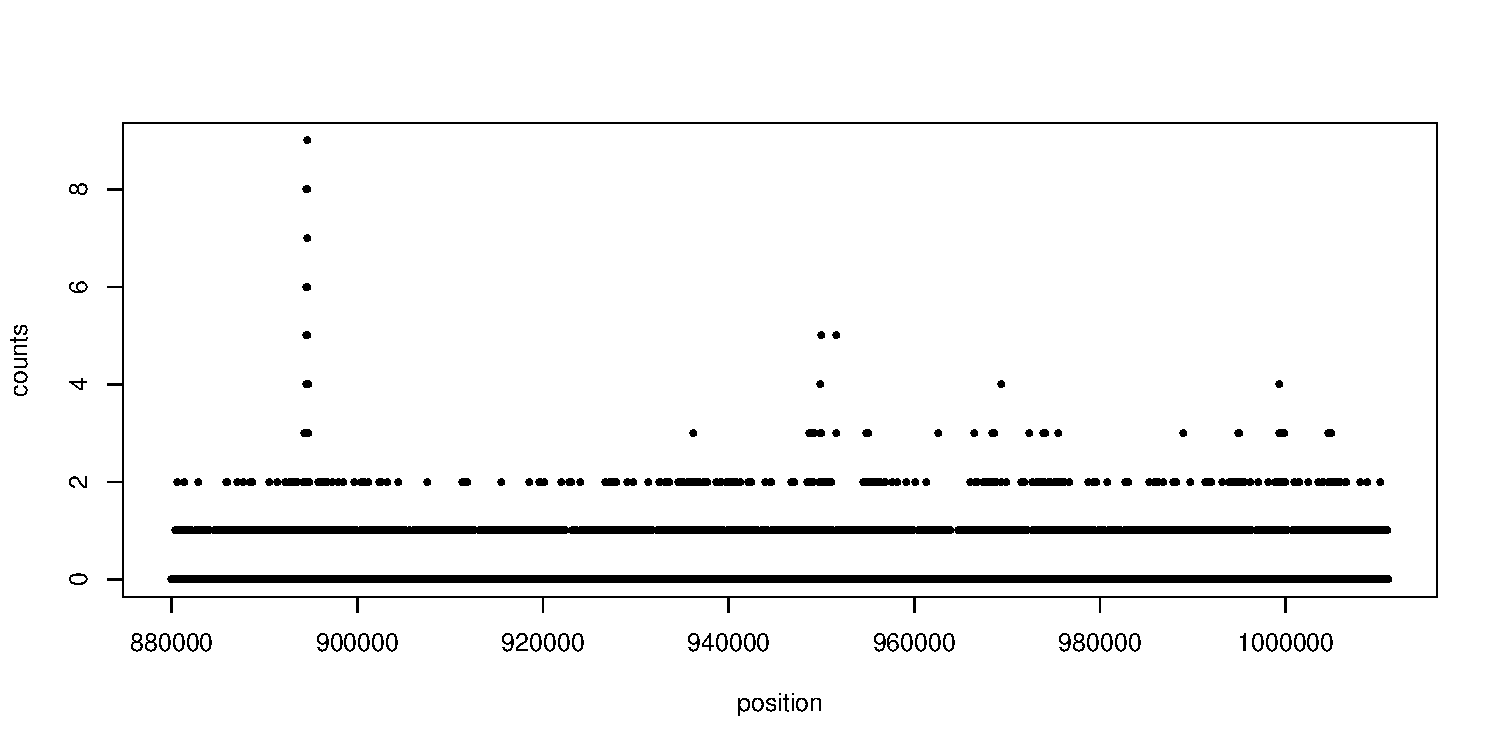
\includegraphics[width=\textwidth]{peaks_comp_a.pdf}
        \caption{}
        \label{fig:seq_peak_data}
    \end{subfigure}
    \begin{subfigure}[b]{0.85\textwidth}
        \centering
        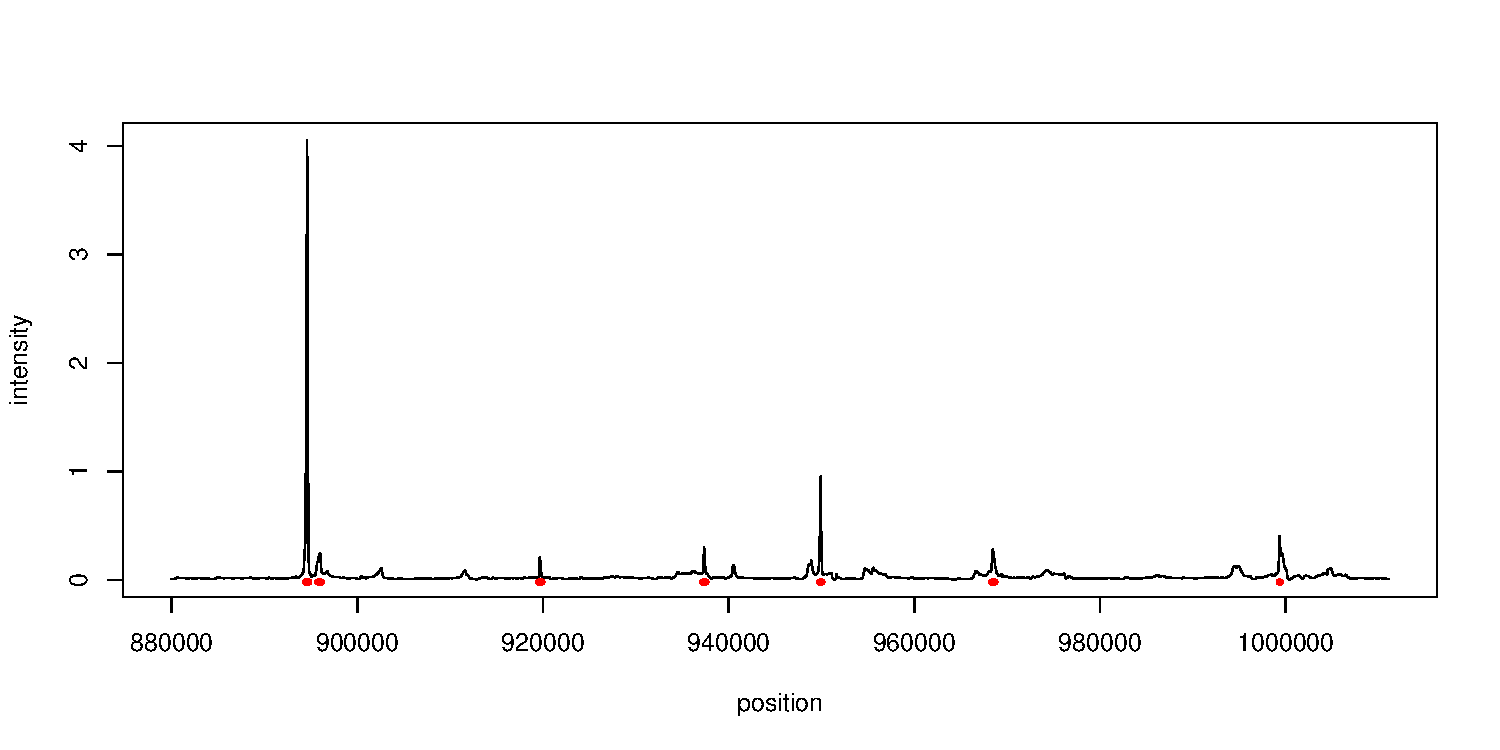
\includegraphics[width=\textwidth]{peaks_comp_b.pdf}
        \caption{}
        \label{fig:seq_peak_est}
    \end{subfigure}
    \caption{Analysis of reads taken from the GM12878 cell line, spanning position 880001 to 1011072 on chromosome 1. (a) Raw sequencing counts. (b) Estimated intensity function from SMASH (black solid line) and location of peaks called by MACS (red markers beneath the estimated intensity).}
    \label{fig:seq_peak}
\end{figure}
From Figure \ref{fig:seq_peak_est} it is clear that SMASH can recognize the peaks detected by MACS. Rather than calling peaks based on certain thresholds however, our method allows users to determine the relative strength and width of each peak, which provides a more comprehensive summary of the sequencing reads. At the same time, SMASH also provides the posterior variances for the intensity estimates, allowing for the option of calling peaks based on thresholds if desired.\\
\section{Discussion}
In this paper we have briefly introduced the adaptive shrinkage method ASH; while it was originally developed in the setting of FDR control for multiple comparisons, we have illustrated its usage as part of two wavelet denoising techniques. Both applications discussed in this paper relax the standard assumption of i.i.d. Gaussian noise, and are thus challenging tasks. Through these applications we are able to demonstrate the flexibility and accuracy of the shrinkage method, revealing its potential in many other applications.

In both the aforementioned applications, our software allows users to easily obtain point estimates for the mean function as well as their approximate posterior variances as a measure of uncertainty. In addition, the variance function can also be estimated, which would provide frequentist confidence intervals for other forms of mean estimation. To the best of our knowledge, there is no readily available software in the wavelet literature that implements joint mean and variance estimation. Simulations have also confirmed that our method is relatively robust to simple forms of autocorrelation between the errors (details needed). In the case of Poisson regression, we improved upon the conjugate Beta priors in Kolaczak (1999) by using ASH as a shrinkage procedure, which allows for more flexibility and precision. %In addition, we have proposed a new procedure to assess the performance of a given method on real datasets without knowing the underlying truth, under the assumption that the data follow a Poisson distribution. 
In both the applications, one further advantage of both our methods is that there is no tuning parameter other than the type of wavelet basis used. On the other hand, the primary resolution level in almost all of the other wavelet-based methods actually affects their performance in varying degrees, depending on the underlying mean and/or variance function. Hence, our fully adaptive procedure allows users to easily apply it to any given dataset, depending on the type of noise.

We have also demonstrated through numerical studies that our methods mostly outperform their respective counterparts from the standard wavelet literature, in terms of pointwise accuracy (MSE in this case). Furthermore, the simplicity of the approximated Gaussian likelihoods as well as the conjugacy of the mixture Gaussian priors imply that our methods are computationally fast, since the posteriors can be computed analytically. In the Gaussian case, simulation results demonstrated that our method is competitive with standard wavelet methods in the case of i.i.d. errors (without explicitly assuming thus), whilst maintaining superior accuracy when heteroskedastic errors are present. Unfortunately, the lack of readily available software (except for MFVB, as described in Menictas \& Wand (2014)) for variance estimation made it difficult to assess the performance of our method in that context. On the other hand, we were able to compare our method to some of the more popular denoising techniques in the Poisson case. Specifically, we have improved upon the conjugate Beta priors used in conjunction with the binomial likelihoods (Kolaczyk (1999)) by using ASH as the shrinkage procedure, which allows for more flexibility and accuracy. This is particularly evident when the mean intensity is low, as is common in many high-throughput genomic sequencing datasets. Our method is also much faster and comparable in accuracy to the popular Haar-Fisz algorithm. Unfortunately, we were not able to directly compare the computational efficiency of our method to many other methods due to differences in the programming software involved.

Although we have only focused on one-dimensional univariate denoising here, our methods can be extended to various scenarios. In the one-dimensional domain, our methods could be used in conjunction with multiple samples, otherwise known as regression analysis of functional data (see Morris (2006)). Instead of dealing with a vector of observations, we perform regression analysis on a matrix of observations, each row of which encapsulates a sample with temporally or spatially structured data points. While Morris (2006) proposed a way to solve a generic regression model, they implicitly assumed the same variance structure for each sample in the same group or category. Our work in the Gaussian case potentially allows for differing variance structures amongst all the samples, thereby relaxing their assumptions. In the simplest case, we could obtain spatially structured differences between groups by including a single covariate that categorizes each sample. In particular, the Poisson model is extremely useful for discovering regions in sequencing reads where structured differences are present between say, various cell lines, as per our sequencing example in the previous section. The Gaussian model could potentially be used in...(??).

With some work, our methods could also be extended to higher dimensions, where a wider range of applications is possible. For example, we could attempt a straight extension to the two dimensional case for both the Gaussian and the Poisson cases as described in Nowak (1998) (again, reference technical report). However, recent research in image denoising problems has shown that smooth curves present in many images such as photographs might render wavelet transformations undesirable. We could thus incorporate ASH into other types of transformations such as curvelets, which would be a potential direction for future work.
\newpage
\section{Reference}

\begin{appendices}
\section{}\label{app:var estimation}\bigskip
\textbf{Variance estimation for Gaussian denoising}

With $\bm{Z}$ as defined in \eqref{eq:varobs1}, we apply the wavelet transform $W$ to $\bm{Z}^2$, and obtain the wavelet coefficients $\bm{\Gd}=W\bm{Z}^2$. Note that $\mathbb{E}(\bm{\Gd})=(\bm{\Gg})$, where $\bm{\Gg}=W\bm{\s}^2$. As with \eqref{eq:likelihood}, we treat the likelihood for $\bm{\Gg}$ as if it were independent, resulting in
\begin{eqnarray}
L(\bm{\Gg}|\bm{\Gd})=\prod_{j=0}^J\prod_{k=0}^{T-1}P(\Gd_{jk}|\Gg_{jk})
\end{eqnarray}
However, the likelihoods $L(\Gg_{jk}|\Gd_{jk})$ are not normal, and have no simple closed form expressions. As such, we approximate the likelihood by a normal likelihood through matching the moments of a normal distribution to the distribution $P(\Gd_{jk}|\Gg_{jk})$ i.e.
\begin{eqnarray}
P(\Gd_{jk}|\Gg_{jk})\approx N(\Gg_{jk},\hat{\mathbb{V}}(\Gd_{jk}))
\end{eqnarray}
so that
\begin{eqnarray}\label{eq:gaus approx}
L(\Gg_{jk}|\Gd_{jk})\approx \phi(\Gd_{jk};\Gg_{jk},\mathbb{V}(\Gd_{jk}))
\end{eqnarray}
where $\phi$ is the normal density function, and $\mathbb{V}(\Gd_{jk})$ is the variance of the detail coefficients. Since these variances are unknown, we estimate them from the data and then proceed to treat them as known. More specifically, since $Z_i\sim N(0,\s_i^2)$, we have that
\begin{eqnarray}
&\mathbb{E}(Z_i^4)\approx 3\s_i^4\notag\\
\label{eq:varvarest}\Rightarrow&\mathbb{V}(Z_i^2)\approx 2\s_i^4
\end{eqnarray}
and so we simply use $\frac{2}{3}Z_i^4$ as an unbiased estimator for $\mathbb{V}(Z_i^2)$. It then follows that $\hat{\mathbb{V}}(\Gd_{jk})$ is given by $\sum_{l=1}^n \frac{2}{3}Z_l^4W_{jk,l}^2$, and is unbiased for $\mathbb{V}(\Gd_{jk})$. These will be the inputs to ASH, which then produces shrunk estimates in the form of posterior means for the corresponding parameters. Although this works well in most cases, there are variance functions for which the above procedure tends to overshrink the detail coefficients at the finer levels. This is likely because the distribution of the wavelet coefficients are extremely skewed, especially when the true coefficients are large (at coarser levels the distributions are much less skewed since we are dealing a linear combination of a large number of data points). One way around this issue is to employ a procedure that jointly shrinks the coefficients $\bm{\Gg}$ and their variance estimates (see JASH). The final estimate of the variance function is obtained from the posterior means via the average basis inverse across all the shifts.

\section{}\label{app:reconstruction}\bigskip
\textbf{Signal reconstruction for Poisson denoising}

Given the posterior means and variances of the $\Ga$'s from ASH, the first step to reconstructing the signal is to find the posterior means of $p_{jk}:=\frac{\Gl_{j+1,2k}}{\Gl_{jk}}$ and $q_{jk}:=\frac{\Gl_{j+1,2k+1}}{\Gl_{jk}}$ (for $j=0,...,J-1$ and $k=0,...,2^j-1$). Specifically, for each $j$ and $k$, we wish to find
\begin{eqnarray}\label{eq:pfromwc1}
&&E(p_{jk})\equiv E\left(\frac{e^{\Ga_{jk}}}{1+e^{\Ga_{jk}}}\right)\\
\label{eq:pfromwc2}&&E(q_{jk})\equiv E\left(\frac{e^{-\Ga_{jk}}}{1+e^{-\Ga_{jk}}}\right)\end{eqnarray}
Given that we already have the posterior expectations and variances for $\Ga_{jk}$, we can approximate \eqref{eq:pfromwc1}-\eqref{eq:pfromwc2} using the Delta method. First, define
\begin{eqnarray}\label{eq:ff}ff(x)=\frac{e^x}{1+e^x}\end{eqnarray}
and consider the Taylor expansion of $ff(x)$ about $ff(E(x))$:
\begin{eqnarray}\label{eq:delta}ff(x)\approx ff(E(x))+ff'(E(x))(x-E(x))+\frac{ff''(E(x))}{2}(x-E(x))^2\end{eqnarray}
where
\begin{eqnarray}
\label{eq:fderiv}&&ff'(x)=\frac{e^x}{(1+e^x)^2}\\
\label{eq:sderiv}&&ff''(x)=\frac{e^x(1-e^{x})}{(1+e^x)^3}
\end{eqnarray}
It is easy to see that
\begin{eqnarray}
&&E(p_{jk})\approx ff(E(\Ga_{jk}))+\frac{ff''(E(\Ga_{jk}))}{2}Var(\Ga_{jk})\\
\label{eq:Ep}&&E(q_{jk})\approx ff(-E(\Ga_{jk}))+\frac{ff''(-E(\Ga_{jk}))}{2}Var(\Ga_{jk})
\end{eqnarray}
noting that we have already computed $E(\Ga)$ and $Var(\Ga)$.

Finally, we can easily back-transform to construct an estimated signal, by noting that we can express $\Gl_i$ as a product of the $p$'s and $q$'s for any $i=1,2,...,n$. Specifically, let $\{c_1,...,c_J\}$ be the binary representation of $i-1$, and $d_m=\sum_{j=1}^m c_j2^{m-j}$ for $j=1,...,J-1$. We then have
\begin{eqnarray}\label{eq:product}\Gl_k=\Gl_{00}p_{00}^{1-c_1}p_{1,d_1}^{1-c_2}...p_{J-1,d_{J-1}}^{1-c_J}q_{00}^{c_1}q_{1,d_1}^{c_2}...q_{J-1,d_{J-1}}^{c_J}\end{eqnarray}
where we usually estimate $\Gl_{00}$ by $\sum_l Y_l$ (see Kolaczyk (1999)). Using the independence of the $p$'s and $q$'s from different scales, we have:
\begin{eqnarray}\label{eq:Eproduct}E(\Gl_i)=\Gl_{00}E(p_{00})^{1-c_1}E(p_{1,d_1})^{1-c_2}...E(p_{J-1,d_{J-1}})^{1-c_J}\notag\\
E(q_{00})^{c_1}E(q_{1,d_1})^{c_2}...E(q_{J-1,d_{J-1}})^{c_J}\end{eqnarray}

As an additional step, we can also construct a credible band around the signal using the posterior variances for inference purposes. From \eqref{eq:product} we have the following:
\begin{eqnarray}\label{eq:E2product}E(\Gl_i^2)=\Gl_{00}^2E(p_{00}^2)^{1-c_1}E(p_{1,d_1}^2)^{1-c_2}...E(p_{J-1,d_{J-1}}^2)^{1-c_J}\notag\\
E(q_{00}^2)^{c_1}E(q_{1,d_1}^2)^{c_2}...E(q_{J-1,d_{J-1}}^2)^{c_J}\end{eqnarray}
To compute the terms in \eqref{eq:E2product}, we again make use of the Delta method (with $ff(x)=(\frac{e^x}{1+e^x})^2$) to obtain:
\begin{eqnarray}
&E(p_{jk}^2)\approx \left(ff(E(\Ga_{jk}))+\frac{ff''(E(\Ga_{jk}))}{2}Var(\Ga_{jk})\right)^2+\notag\\
& \hspace{1.5 in}\{ff'(E(\Ga_{jk}))\}^2Var(\Ga_{jk})\\
&E(q_{jk}^2)\approx \left(ff(-E(\Ga_{jk}))+\frac{ff''(-E(\Ga_{jk}))}{2}Var(\Ga_{jk})\right)^2+\notag\\
& \hspace{1.5 in}\{ff'(E(-\Ga_{jk}))\}^2Var(\Ga_{jk})
\end{eqnarray}
Finally we combine \eqref{eq:Eproduct} and \eqref{eq:E2product} to find $Var(\Gl_k)$, which allows us to construct credible intervals.

Note here that for the reconstructed signal to possess the property of shift invariance (see Coifman \& Donoho (1995)), the $\Ga$'s are extracted from a so-called translation invariant (TI) table (see Coifman \& Donoho (1995), and Kolaczyk (1999)) rather than as described above. The idea remains the same however, and we can simply think of the extra $\Ga$'s as being defined similarly as the original $\Ga$'s, albeit from a shifted version of the original data points. To be more specific, the TI table contains the $\Ga_{jk}$ for all circulant shifts of the signal. Here we define the $t$-th shift of the signal $\bm{Y}$, denoted by $\bm{Y}^{(t)}$, to be created from $\bm{Y}$ itself by moving the first $n-t$ elements of $\bm{Y}$ $t$ positions to the right and then putting the last $t$ elements of $\bm{Y}$ in the first $t$ locations. Using this table, we are essentially computing the posterior expectations in \eqref{eq:Eproduct}-\eqref{eq:E2product} by averaging over all posterior expectations for every shift of the original signal ie.
\begin{eqnarray}
\label{eq:TIapproxexp}\frac{1}{n}\sum_{t=1}^n E(\hat{\Gl}_k^{(t)})
\end{eqnarray}
which is an approximation to the true quantity we wish to compute, given by
\begin{eqnarray}
E(\hat{\Gl}_k)=\sum_{t=1}^n E(\hat{\Gl}_k^{(t)})P(\mbox{$t$-th shift})
\end{eqnarray}
\end{appendices}
\end{document}
